%\documentclass[manuscript,natbib]{aastex}
\documentclass[12pt,preprint]{aastex}

%%\newcommand{\vdag}{(v)^\dagger}
\newcommand{\bvf}{Brunt-V\"ais\"al\"a }
\newcommand{\teff}{$\rm T_{eff}$}
\newcommand{\logg}{$\log$\ g }
\newcommand{\kic}{KIC }
\newcommand{\kicnsp}{KIC}
\newcommand{\sigrms}{$\sigma_{\rm RMS}$}
\newcommand{\mstar}{$M_*$}
\newcommand{\menv}{$M_{\rm env}$}
\newcommand{\mhe}{$M_{\rm He}$}
\newcommand{\xo}{$X_o$}
\newcommand{\qfm}{$q_{\rm fm}$}
\newcommand{\muHz}{\mbox{$\mu$Hz}}
\newcommand{\msun}{$M_\odot$}

\shorttitle{Asteroseismology of GD358}
\shortauthors{Bischoff-Kim}
\usepackage{graphicx}
%\usepackage{array} %Don't activate - doesn't play nice with deluxe tables!!!
\usepackage{epsfig}
\usepackage[outdir=./]{epstopdf}
%\usepackage{ulem}
%\usepackage{booktab}
%\usepackage{natbib}

%\bibliographystyle{natbib}

\begin{document}   


\title{Asteroseismology of GD358 with complex C/O core profiles}

\author {Agn\`es~Bischoff-Kim\altaffilmark{1},
J.~L. Provencal\altaffilmark{2,3},
M.~H.~Montgomery\altaffilmark{3,4},
H.~L. Shipman\altaffilmark{2,3},
Samuel~T.~Harrold\altaffilmark{4},
B.~Howard\altaffilmark{3},
W.~Strickland\altaffilmark{5},
D.~Chandler\altaffilmark{5},
D.~Campbell\altaffilmark{5},
A.~Arredondo\altaffilmark{5},
R.~Linn\altaffilmark{5},
D.~P.~Russell\altaffilmark{5},
D.~Doyle\altaffilmark{5},
A.~Brickhouse\altaffilmark{5},
R.~Linn\altaffilmark{5},
D.~Peters\altaffilmark{5},
P.~A. Bradley\altaffilmark{6},
S.-L. Kim\altaffilmark{7},
X.~J.~Jiang\altaffilmark{8},
Y-N.~Mao\altaffilmark{8},
A.~V.~Kusakin\altaffilmark{9},
A.~V.~Sergeev\altaffilmark{10,11},
M.~Andreev\altaffilmark{10,11},
A.~Maksim\altaffilmark{10,11},
S. Velichko\altaffilmark{12},
R.~Janulis\altaffilmark{12},
E.~Pakstiene\altaffilmark{12},
F.~Ali\c cavu\c s\altaffilmark{13},
N. Horoz\altaffilmark{13},
S.~Zola\altaffilmark{14,15},
W.~Og{\l}oza\altaffilmark{14,15},
D.~Koziel-Wierzbowska\altaffilmark{14,15},
T.~Kundera\altaffilmark{14,15},
D. Jableka\altaffilmark{14,15},
B. Debski\altaffilmark{14,15},
A. Baran\altaffilmark{15},
S. Meingast\altaffilmark{16},
T. Nagel\altaffilmark{17},
L. Loebling\altaffilmark{17},
C. Heinitz\altaffilmark{17},
D. Hoyer\altaffilmark{17},
Zs. Bogn\'ar\altaffilmark{18}
}
\altaffiltext{1}{Penn State Worthington Scranton, Dunmore, PA 18512; axk55@psu.edu}
\altaffiltext{2}{University of Delaware, Department of Physics and Astronomy
Newark, DE 19716; jlp@udel.edu}
\altaffiltext{3}{Delaware Asteroseismic Research Center, Mt. Cuba Observatory,
Greenville, DE 19807}
\altaffiltext{4}{Department of Astronomy, University of Texas, Austin, TX 78712;
mikemon@rocky.as.utexas.edu}
\altaffiltext{5}{Meyer Observatory and Central Texas Astronomical Society, 209
Paintbrush, Waco, TX 76705; chandler@vvm.com}
\altaffiltext{7}{Korea Astronomy and Space Science Institute, Daejeon 34055, Korea}
\altaffiltext{8}{National Astronomical Observatories, Academy of Sciences, Beijing 10012, People's Republic of
China; xjjiang@bao.ac.cn}
\altaffiltext{9}{Fesenkov Astrophysical Institute, Almaty 050020, Kazakhstan}
\altaffiltext{10}{Ukrainian National Academy of Sciences, International Center for Astronomical,
Medical and Ecological Research, 27, Akademika Zabolotnoho Ave., 03680 Kyiv, Ukraine; sergeev@terskol.com }
\altaffiltext{11}{Russian Academy of Sciences, Institute of Astronomy, Terskol Branch, 81, Elbrus Ave., ap. 33, Tyrnyauz,
Kabardino-Balkaria Republic, 361623, Russian Federation; sergeev@terskol.com}
\altaffiltext{12}{Institute of Theoretical Physics and Astronomy, Vilnius
University, Vilnius, Lithuania; jr@itpa.lt}
\altaffiltext{13}{Ulupinar Observatory, \c Canakkale Onsekiz Mart University, Turkey}
\altaffiltext{14}{Astronomical Observatory of the Jagiellonian University, ul. Orla
171, 30-244 Cracow, Poland; szola@oa.uj.edu.pl}
\altaffiltext{15}{Mount Suhora Observatory, Cracow Pedagogical University, Ul.
Podchorazych 2, 30-084 Krakow, Poland; zola@astro1.as.ap.krakow.pl}
\altaffiltext{16}{Institut f\H ur Astrophysik, Universit\H at Wien, T\H urkenschanzstrasse 17, 1180 Wien, Austria}
\altaffiltext{17}{Institut fuer Astronomie und Astrophysik, Kepler Center for Astro and Particle Physics,
Eberhard Karls Universitaet Tuebingen, Sand 1, 72076 Tuebingen Germany; nagel@astro.uni-tuebingen.de}
\altaffiltext{18}{Konkoly Observatory, MTA CSFK, Konkoly Thege M. u. 15-17, H-1121 Budapest, Hungary}

\clearpage
\newpage

\begin{abstract}
We report on the analysis of 34 years of photometric observations of the pulsating
helium atmosphere white dwarf GD358.  The complete data set includes archival data from 1982-2006, 
and 1195.2 hours of new observations from 2007-2016. From this data set, we extract 15 frequencies 
representing g-mode pulsation modes, adding 4 modes to the 11 modes 
known previously. We present evidence that these 15 modes are $\ell=1$ modes, 13 of which belong to 
a consecutive sequence in radial overtone
$k$. We perform a detailed asteroseismic analysis using models that include parameterized, complex carbon and oxygen 
core composition profiles to fit the periods. Recent spectroscopic analyses place GD358 near the red edge of the DBV instability strip, at 24,000 $\pm$ 500~K and a \logg of 7.8 $\pm$ 0.08 dex. The surface gravity translates to a mass range of 0.455 to 0.540 \msun. Our best fit model has a temperature of 23,650~K and a mass of 0.5706 \msun ~. That is slightly more massive than what the most recent spectroscopy suggests. We find a pure helium layer mass of $10^{-5.50}$, consistent with the outward diffusion of helium over time.

\end{abstract}

\keywords{Stars: oscillations --- Stars: variables: general --- white dwarfs}

\section{Astrophysical Context}
\label{intro}
White dwarfs are the end product of evolution for around 98\% of the stars in our Galaxy. 
Buried in their interiors are the records of physical processes that take place during 
earlier stages in the life of the star. Nuclear reaction rates during the core helium 
burning phase set the core composition of white dwarfs, while the relative time spent 
burning hydrogen and helium during the asymptotic-giant-branch (AGB) phase and mass-loss 
episodes determine the thickness of the helium layer \citep{Lawlor06,Althaus05}. Helium 
atmosphere white dwarfs (DBs) comprise roughly 20\% of the population of field white 
dwarfs, with most of the remaining 80\% consisting of their hydrogen atmosphere (DA) 
cousins. One theory behind the bifurcation into two spectral classes is that during post-AGB evolution, a very late thermal pulse can burn off the residual hydrogen 
in the envelope, producing a nearly pure helium atmosphere \citep{Iben83}. Such objects 
then return to the white dwarf cooling track as PG 1159 stars, which are 
widely believed to be the precursors of most DB white dwarfs. DBs are found to pulsate at 
effective temperatures ranging between 21,000 K and 28,000 K \citep{Beauchamp99, Castanheira05}. 

The subject of this paper, GD358 (V777 Her) is the brightest ($m_{\rm v}=13.7$) and best 
studied helium atmosphere white dwarf pulsator. It is located near the red edge of the 
instability strip, with a spectroscopic temperature of \teff\ $=24000\pm500$ ~K and \logg\ $=7.8$ 
\citep{Nitta12, Koester2013}. GD358's pulsation spectrum contains a series of independent 
radial overtones, many with complex frequency structure.  For one epoch of data taken during a WET run, models involving magnetic fields and oblique rotation have been proposed to explain such structure \citep{Montgomery10}.

Since the 2006 Whole Earth Telescope (WET) run reported in \citet{Provencal09}, 
we have maintained an active observing program of GD358 in an effort to identify additional
frequencies in this complex star. These new observations have identified additional 
periods in GD358's pulsation spectrum, bringing the total known independent radial overtones to 15. Thirteen of 
these modes belong to a consecutive $\ell=1$ sequence, the longest sequence observed 
in a DBV. 

Paradoxically, among the DBVs with enough detected periods to be fitted 
asteroseismically, GD358 is the only one that has not been analyzed using the complex 
C/O profiles adapted and parameterized from stellar evolution calculations
(e.g. {}\citet{Salaris97,Althaus05}). The most recent fits of GD358 \citep{Metcalfe03c} were 
performed using 11 observed modes and simple models where the oxygen abundance 
drops linearly from its central value to zero. We present here a new detailed asteroseismic analysis 
of GD358, taking advantage of its long sequence of $\ell=1$ modes to better constrain 
the asteroseismic fits and define the limits of high precision white dwarf asteroseismology.  

The present analysis also allows us to place GD358 in the context of stellar evolution. 
According to the models, the precursors of DBs emerge from the born-again phase with 
envelopes containing a nearly uniform mixture of helium (He), carbon (C), and oxygen (O) 
out to the photosphere \citep{Dreizler98,Herwig99}. As the PG 1159 stars cool, the helium 
diffuses upward and gradually accumulates to form a chemically pure surface layer. Through 
the DBV instability strip, this process is still ongoing so that instead of a pure helium 
layer surrounding the carbon and oxygen core, one has a region where the carbon and helium 
are still mixed. This leads to a double layered structure, with the pure He surface layer 
overlying the remainder of the uniform He/C/O envelope, all above the degenerate C/O core. 
A key prediction of the diffusion models is that, for a given stellar mass, the pure He 
surface layer will steadily grow thicker as the DB star cools.  GD358 is the fourth DBV 
we can use to check this theory. The other three DBVs 
(\citet{Bischoff-Kim14,Sullivan08, Metcalfe03c}) have painted a picture qualitatively consistent with 
the diffusion calculations, with the hotter best fit models having thinner pure helium 
layers. With GD358, we seek to confirm this trend.

In Section \ref{data}, we present our new observations and outline the data reduction process.  
In Section \ref{freq}, we establish the framework for frequency identification, and present the 
list of frequencies used for the asteroseismic investigation. We perform further analysis of the observed 
frequencies in Section \ref{analysis}, and motivate the $\ell$ and $m$ identification of the modes. 
We present the asteroseismic fitting of GD358's pulsation spectrum in section \ref{fitting}, present 
the results in section \ref{results} and discuss our results in section \ref{discussion}.

\section {New Observations and Data Reduction}\label{data}

GD358 was discovered in 1982 \citep{Winget82} and has been the target of the Whole 
Earth Telescope (WET) in 1990, 1994, 2000, and 2006 \citep{Provencal09, Kepler03,Winget94}. 
New observations presented here include 278 individual observing runs (1105.1 hrs) spanning 
2007-2016 (Table \ref{journal}). Each season of observations was obtained as part of 
multi-site WET campaigns \citep{wet90}. 

Data reduction follows the steps described in \citet{Provencal12}. In brief, the new observations 
were obtained with CCD photometers at multiple sites, each with distinct effective bandpasses. 
We reduce the bandpass issues by using CCDs with similar detectors whenever possible and 
employing a red cutoff filter (BG40 or S8612) to normalize wavelength response and 
minimize extinction effects. We corrected each image for bias and thermal noise, and 
normalized by the flat field. Aperture photometry using the Maestro photometry pipeline 
described by \citet{Dalessio10} was performed on each image, covering a range of 
aperture sizes for the target and comparison stars. For each individual nightly run, we 
chose the combination of aperture size and comparison star(s) producing the highest 
signal/noise light curve. 

We used the WQED pipeline \citep{wqed} to examine each light curve for photometric 
quality, remove outlying points, divide by suitable comparison stars, and correct for 
differential extinction. This observational technique is therefore not sensitive to 
oscillations longer than a few hours. The final product is a series of light curves 
with amplitude variations represented as fractional intensity (mmi). The unit is a linear 
representation of the fractional intensity of modulation (1 mmi $\approx$ 1 mmag). We present
our Fourier transforms (FTs) in units of modulation amplitude 
($1\ {\rm mma}=1 \times 10^{-3}\ {\rm ma} = 0.1 \% = 1\ {\rm ppt}$).

The final reduction step is to combine the individual light curves 
(an example is shown in Fig. \ref{tersk}) to produce complete light curves for GD358 for each 
observing season. As we do for all white dwarf pulators, we assume GD358 oscillates around 
a mean light level. This assumption allows us to assess overlapping light curves from multiple 
telescopes and identify and correct any vertical offsets. As discussed in detail in \citet{Provencal09}, we find 
no significant differences between the noise levels of amplitude spectra using: 
1) the combination of all light curves including overlapping 
segments from different telescopes, 2) the combination of light curves where we retain 
only higher signal to noise observations in overlapping segments and 3) combining all light 
curves using data weighted by telescope aperture.

\begin{figure}
\epsscale{0.7}
\plotone{terskol}
\caption{Light curve of GD358 obtained with the Peak Terksol 2.0 m telescope.  Each point corresponds 
to a 10 s exposure. The nonlinear, multiperiodic nature of this star is clearly evident.
(A color version of this figure is available in the online journal.)
\label{tersk}
}
\end{figure}

The complexities associated with GD358's pulsations (see Section \ref{freq}) led us to also 
re-reduce all available archival data \citep{Provencal09, Bradley04, Kepler03, Winget94, Winget82} to
insure continuity in methodology. The final result is a series of light curves 
for each observing season between 1982 and 2016. 
For the new observations, 2007 contains 8.1 hrs of observation, 2008 26.1 hrs, 2009 45 hrs, 
2010 201.3 hrs, 2011 401.1 hrs, 2012 150.5 hrs, 2013 87 hrs, 2014 184.6 hrs, 2015 55 hrs and 2016 90.6 hrs. 
Our coverage is not complete, and this incompleteness produces spectral leakage in the 
amplitude spectra. To quantify this, our standard procedure samples single sinusoids using exactly the 
same times as the original data for each season. The resulting amplitude spectrum, 
or ``spectral window'', is the pattern produced in the FT by a single frequency. 
The FTs for 2010, 2011, and 2014 are given in Fig.~\ref{fts}.


\begin{figure}
\plotone{gd358multidft}
\caption{Fourier Transforms of GD358 for the 2010, 2011, and 2014 observing seasons.
The frequency range of the observed series of $\ell=1$ modes discussed in Section \ref{analysis} 
is indicated by the left arrow (red).  Peaks below $\approx$ 2400 \muHz\ are combination 
frequencies discussed in Section \ref{mode} (right arrow, blue). 
(A color version of this figure is available in the online journal.)
\label{fts}
}
\end{figure}

\section{Frequency Identification}\label{freq}
 
Our goal is to compile a complete list of GD358's observed independent and combination frequencies 
to be used in a comprehensive asteroseismic analysis. GD358 is known for large scale changes in 
amplitudes and small but not insignificant frequency variations on a variety of timescales 
\citep{Provencal09, Kepler03}.  The amplitude and frequency variations evident in Fig.~\ref{fts} demonstrate that 
it is not feasible to analyze the entire data set as one unit. To minimize the effects of the long term  
amplitude and frequency variations, we analyze the light curves from each observing season individually.

We use {\sl Period04} \citep{Lenz05} for Fourier analysis and nonlinear least squares fitting to 
identify statistically significant frequencies in each FT. We adopt the criterion that a peak must have 
an amplitude at least four times that of the average noise level in the given frequency range 
\citep{Provencal12}. This criterion places a 99.9\% probability that the peak represents a real signal,
and is not a result of random noise \citep{Scargle82, Provencal12}.  We define ``noise'' as the frequency-dependent 
average amplitude after prewhitening of the dominant frequencies. This is unquestionably a conservative estimate, 
as it is impractical to assume that the complete set of ``real'' frequencies are removed when determining
the noise level. This is inarguably true for GD358, where amplitude modulation is present, and the peaks above $\approx$ 2500 $\mu$Hz\ 
are combination frequencies (see Section \ref{mode}, \citet{Provencal09}).  Fig.~\ref{noise} displays the average noise 
as a function of frequency for the 2007-2016 observing seasons. A similar plot for the 
archival data is presented in Fig. 3 of \citet{Provencal09}. We also calculated Monte Carlo 
simulations using the routine provided in {\sl Period04}.  This routine generates a set of light curves using 
the original times, the fitted frequencies and amplitudes, and added Gaussian noise. A least squares fit is 
performed on each simulated light curve, with the distribution of fit parameters giving the uncertainties. 
Our Monte Carlo results are consistent with our average noise estimates.

\begin{figure}
\plotone{noise}
\caption{A comparison of the average noise as a function of frequency for the 2007-2016 observing 
seasons.  Each data set was prewhitened by its dominant frequencies.  The noise levels for each 
season are somewhat different.  This must be taken into account during frequency analysis.  
\label{noise}
}
\end{figure}

Having established our baseline noise levels, we proceed to frequency selection and identification.
Our standard frequency selection procedure identifies the largest amplitude resolved peak in the FT,
fits a sinusoid with that frequency to the data set, subtracts the fit from the light curve, 
recomputes the FT, examines the residuals, and repeates the process until no significant power 
remains. This technique is known as prewhitening. Prewhitening has inherent dangers, and must be 
employed with extreme vigilance, especially as we are aware of amplitude and/or frequency 
modulation in our data set. A detailed discussion of the prewhitening procedure and steps 
taken to minimize the effects of amplitude modulation is given in \citet{Provencal09}. Our final 
identifications of independent frequencies detected in each observing season are given in 
Table \ref{freq1} and Table \ref{freq2}.

\section{Frequency Analysis}\label{analysis}

\subsection{Frequency Distribution}
Perusal of Tables \ref{freq1} and \ref{freq2} shows that GD358's observed frequencies vary in two
important ways.  First, frequencies detected in a given observing season are not found 
in all observing seasons. Asteroseismology is based on the assumption that the available pulsation
frequencies are linked to stellar structure.  Since we are fairly certain that GD358's internal structure 
does not change on the timescales of the observations, we can assume that GD358 excites 
different subsets of its available pulsations at different times. While this is a common phenomenon
seen in white dwarf pulsators, the selection mechanism remains unknown. The best way to 
determine GD358's complete set of pulsation frequencies is to combine frequency identifications 
from multiple observing seasons as outlined in \citet{Kleinman98}.  

\begin{figure}
\epsscale{0.9}
%\plottwo{gd358multif_2015.eps}{gd358multi.eps}
%\centering{
%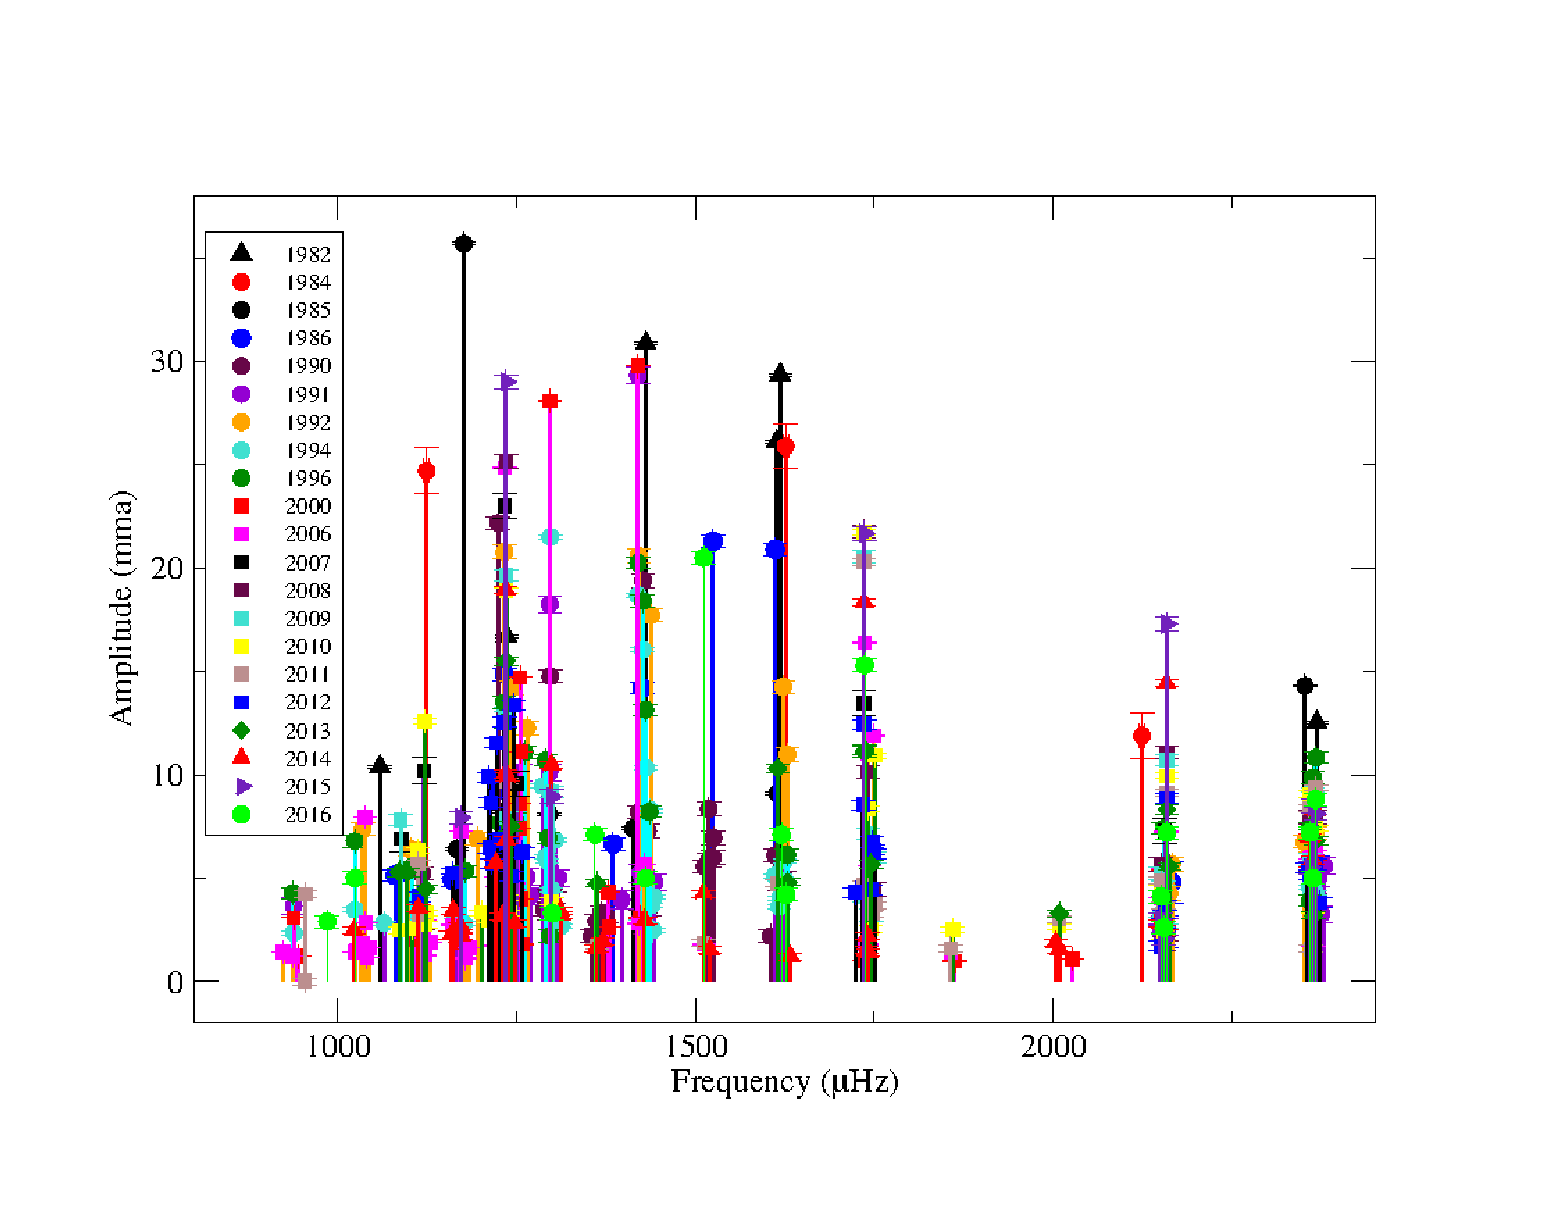
\includegraphics[width=1.0]{gd358multif_2015.eps}
%}
\plotone{gd358multif_2015.eps}
\caption{A schematic representation of GD358's pulsation modes for all available data between
1982 and 2015. Systematic patterns of distribution are evident. The bands between 2400 and 1000
\muHz\ (400 and 1000 s) are of particular importance for this work. (A color version of this 
figure is available in the online journal.)
\label{schematic}
}
\end{figure}

Fig.~\ref{schematic} presents a schematic representation of GD358's 
independent frequencies detected between 1982 and 2016.  
The features of asteroseismic importance are the localized bands between 900 and 2400
\muHz\ (1100 and 400 s). We interpret the bands to represent a series of modes of radial overtone $k$. The bands
themselves illustrate the second way in which GD358's frequencies vary. Each band consists of 
frequency detections from multiple observing seasons, but each band is significantly wider in 
frequency space than the frequency error of any single measurement, arguing that some process 
is acting on the frequencies. The simplest explanation is rotational splitting.  However, with the 
exception of the two highest frequency (shortest period) bands ($k=8$ and $k=9$ 
from \citet{Provencal09}), we find no clear evidence of stable multiplet structure in the frequency 
distributions of the lower frequency (longer period) bands (Fig.~\ref{rot}). This does not imply that the 
structures found by \cite{Winget94}, \cite{Kepler03}, \cite{Montgomery10} and others are not real. In 
particular, it is clear that the 1741 \muHz\ ($k=12$) mode can be explained by the oblique rotation model during 2006. However, 
previous work represents short snapshots of GD358. When examined over timescales of decades, these structures 
do not regularly recur, and so cannot be interpreted as simple rotational splitting. The lower frequency band widths 
are most likely the result of unknown processes that obscure any 
underlying signatures of simple rotational splitting. 
\begin{figure}
 \epsscale{1.0}
 \plotone{gd358k17_k8.eps}
% \plottwo{gd358multifk17.eps}{gd358multifk8.eps}
 \caption{The detailed schematic distribution of frequencies for the bands near 1300({\em{right}}
 and 2360 \muHz\ ({\em{left}}). As an example of the higher frequency bands, the 1300 \muHz\ band 
 shows no multiplet structure, unlike the 2360 \muHz\ band. Here we see clear evidence of multiplet 
 structure. Assuming the triplet represents
 $\ell=1$, this implies a rotation period of $\approx 1.5$ days. Note changes in the x scale for both axes.
 (A color version of this figure is available in the online journal.)
 \label{rot}}
\end{figure}

Fig. \ref{schematic} also shows that the widths of the bands are not constant, but change 
from band to band. \citet{Bell15} presents an interesting analysis of the hydrogen atmosphere pulsator 
(DAV) KIC4552982, in which they identify 17 bands of pulsation frequencies. KIC4552982 is one of the 
coolest ZZ Cetis known \citep{Tremblay2013}, and it follows the general pattern exhibited 
by GD358: the highest frequency (shortest period) mode shows evidence of rotational splitting, while the 
lower frequency (longer period) modes are complex bands. The authors note that this DAV's bands have 
different widths in frequency space, and that there may be astronomical significance to this. 
Although the observational timebases and coverage are quite different (20 continuous months 
for KIC4552982 vs 34 incomplete years for GD358), our data presents the opportunity to investigate this 
for a cooler DB pulsator.  We measured the widths of each of GD358's band where we have
more than 10 detections. We define ''width'' as the difference between the lowest and highest frequency 
detected in each band. Fig. \ref{thick} presents the results. We find no correlation of width with number
of detected peaks in each band. Interestingly, the widths of GD358's bands are commensurate with those 
found in KIC4552982. We find a general increase in width with decreasing frequency (increasing period), 
until we reach the band at 1238 \muHz\ (807 s). This band has a width at least twice as wide as any other. 

\citet{Mont2016} recently outlined a possible explanation for the behavior seen in the low frequency modes
of these cool DAVs that should also apply to GD358. White dwarfs pulsate in nonradial g-modes. As a DBV such as 
GD358 pulsates, it experiences local surface temperature variations as large as 3000 K.  The temperature 
variation affects different modes in different ways.  An appropriate analogy is to consider each mode's 
propagation region as a box with a lid. The box is defined as the region where the mode frequency is 
less than both the buoyancy (Brunt-V{\"a}is{\"a}l{\"a}) and acoustic (Lamb) frequencies.  The box's lid 
represents the mode's outer turning point. For short period modes (such as $k=8$ and $k=9$ in GD358), the 
lid is defined by the acoustic frequency, which is relatively insensitive to surface temperature variations. 
As the star pulsates, the box will not change, so these modes should be stable.  For the longer period modes, 
the lid of the box is defined by the buoyancy frequency, which goes to zero at the base of the surface 
convection zone. This is the important point: for longer period modes, the box lid
is actually defined by the base of the convection zone, which is very sensitive to local temperature variations.  
As GD358 pulsates, its convection zone deepens and thins in response to the local temperature variations. 
In our analogy, the lid of the box moves, effectively changing the characteristics of the box. Long period modes with 
outer turning points defined by the base of the convection zone should be perturbed and this is indeed 
what we see in GD358. 

An additional interesting behavior is given by the distribution of average amplitudes for the bands 
(Fig~\ref{schematic}). In particular, the two bands at 1857.7 and 2007.6  \muHz\ have never been observed 
at amplitudes above 4 mma. The band at 1369 \muHz\ is also only observed at lower amplitudes. Interestingly, 
the band at 1741.5 \muHz\ was not observed at large amplitude prior to 2006, and it has remained at high 
amplitude since that time. 

To summarize this section in broad brush strokes, the observed global pulsations involve the whole star, 
but each pulsation samples the star in slightly different ways.  Modes with lower frequencies 
(higher radial $k$ values) preferentially sample the outer layers, while modes with higher frequencies 
(lower radial $k$ values) have outer turning points that are farther from the surface, and so sample the 
deeper interior. It makes intuitive sense that lower frequency modes would be affected by processes 
confined to the outer stellar atmosphere, such as the convection zone. We speculate that the 
observed band widths and pulsation amplitudes contain information about the convection zone and/or any surface
magnetic field. Further investigation requires guidance from theory.  


\begin{figure}
 \epsscale{0.8}
 \plotone{modethick.eps}
 \caption{Width of each bank of power in Fig.~\ref{schematic}. We find an overall increase 
 in band thickness with decreasing frequency (increasing period).  The band at 807~s has a width
 at least twice as large as other bands.  
 \label{thick}}
\end{figure}


\subsection{Mode Identification}\label{mode}
Our current work has produced a well defined sequence of modes, adding to 
previous studies \citep{Montgomery10, Provencal09, Metcalfe00, Winget94}. The previous 
identification of these modes as a series of $l$=1 radial overtones is based mostly on 
the pulsation frequency distribution and limited spectroscopic analysis 
\citep{Kotak02, Castanheira05}. It is important to further investigate these identifications 
as we initiate an in depth asteroseismic investigation.  

GD358's combination frequencies provide a tool by which we can bolster $\ell$ identifications. 
Combination frequencies are typically observed in the FTs of moderate to large amplitude pulsators.  
They are identified by their exact numerical relationships with parent frequencies.  
The combinations themselves are not independent, but result from nonlinear effects associated 
with the surface convection zone \citep{Brickhill92, Brassard95, Wu01, Ising01}.  
\citet{Wu01} lays the groundwork, showing that observed amplitudes of the combination 
frequencies depend on geometric factors such as the $(\ell,m)$ indices of the parents and the 
inclination of the pulsation axis to the line of sight.  

The methods outlined in \citet{Provencal12} and \citet{Montgomery10} work best when applied to 
larger amplitude frequencies detected in high signal to noise data sets such as provided by 
extensive WET runs.  The primary reason for this is that combination frequencies are lower 
amplitude than their parents, and so are more difficult to detect in sparse data.  We chose 
the 1990, 1994, 2006, 2010, 2011, and 2014 observing seasons, and looked at pulsation 
frequencies with amplitudes above 10 mma.  

As an example, Fig.~\ref{modeamps} shows the probability distribution of $\ell$ and $m$ 
values for the 1735.96 \muHz\ frequency as detected in 2014. To produce the distribution, we ran
the amplitude code \citep{Montgomery10} 1000 times, and selected the results having $Res_{rms}<9.5\times10^{-06}$, 
where $Res_{rms}$ are the root-mean-squared residuals between predicted and observed amplitudes.  
For our example, this mode is clearly preferred as an $\ell=1$, $m=1$ mode. We find similar results for all
modes above 10 mma in the 1990, 1994, 2006, 2010, and 2014 observing seasons. Combining the results from the 
combination frequencies with previous evidence, we are confident that the bands in Fig.~\ref{schematic} represent
a series of $\ell=1$ modes.  

\begin{figure}
 \epsscale{0.8}
 \plotone{modeamps.eps}
 \caption{Probability distribution (from 0 to 1) of $\ell$ and $m$ values for the 1735.96 variation detected in 
 2014.  The distribution is produced from 1000 simulations, selecting with $Res_{rms}<9.5^{-06}$. 
 The amplitudes of the observed combination frequencies argue that this is $\ell=1$, $m$=1.  
 \label{modeamps}
 }
\end{figure}

%isnt' that same as table \ref{gd}?

Finally, given the $l$=1 identification and the lack of definitive multiplet structure for the lower 
frequency modes, the best way to determine the central frequency for each band is simply to 
average the detected frequencies in the bands.  We experimented with numerous weighting techniques, 
and determined there is no significant difference in our solutions.  Our final frequencies for each band 
are given in Table~\ref{gd}. We use these periods in our asteroseismic fitting. 

\section{Asteroseismic fitting}
\label{fitting}

The basic method in our asteroseismic fitting consists of calculating grids of white dwarf models and 
running a fitting subroutine to match the periods of the models ($\rm P^{calc}$) with the observed 
periods $P^{\rm obs}$. Following standard statistical methods, each fit is assigned a fitness 
parameter calculated the following way:

\begin{eqnarray}
\label{fiteq1}
\sigma_{\rm RMS} = \sqrt{\frac{1}{W} \sum_{1}^{n_{\rm obs}} {w_i(P^{\rm calc}_i-P^{\rm obs}_i)^2}}, \\
W=\frac{n_{\rm obs}-1}{n_{\rm obs}}\sum_{1}^{n_{\rm obs}}w_i
\end{eqnarray}

\noindent where $n_{\rm obs}$ is the number of periods present in the pulsation spectrum and the weights $w_i$ 
are the inverse square of the uncertainties listed for each period in table \ref{gd}. We note that the two 
shortest period modes have 6000 times the weight of the longest period mode. Another way to think about this 
is to assume that we have a calculated period that matches the highest period mode very poorly, 
being 20 seconds away. 20 seconds is roughly half the average period spacing for $\ell=1$ modes in the 
relevant area of parameter space and so it is the worse period fit one can get. In order to have the 
same impact on $\sigma_{\rm RMS}$, the lowest period mode would have to match to within 0.26 seconds. 
In essence this is almost ignoring the modes that have a period measurement uncertainty of 0.5~s or more. 
It is, however completely consistent with the relative uncertainty on the periods and it provides us with 
a true measure of the goodness of fit, while accounting for all the data we have.

\subsection{The Models}
\label{models}

To compute our models, we used the White Dwarf Evolution Code (WDEC). The WDEC uses hot  and self-consistently allows them to relax to be solutions of the equations of stellar structure with the temperature of our choice.
polytrope models with temperatures above 100{,}000~K as starting model and numerically evolves them until they are thermally relaxed 
solutions to the stellar structure equations and have the temperature of our choice. The mass is also fixed as an input, and so is the internal chemical composition profiles (no mass loss, no time dependent diffusion of elements). Each model we compute for our grids is the result 
of such an evolutionary sequence. The WDEC is described in detail in \citet{Lamb75} and 
\citet{Wood90}. We used smoother core composition profiles and implemented more complex profiles 
that result from stellar evolution calculations \citep{Salaris97}. We updated the envelope 
equation of state tables from those calculated by \citet{Fontaine77} to those given by 
\citet{Saumon95}. We use OPAL opacities \citep{Iglesias96} and plasmon neutrino rates 
published by \citet{Itoh96}. 

DBVs are younger than their cooler cousins the DAVs. Time-dependent diffusion calculations 
\citep[e.g.][]{Dehner95,Althaus05} show that at 24{,}000~K, a typical temperature for a DBV, 
the carbon has not yet fully settled into the core of the star. We expect the helium layer to 
be separated into a mixed He/C layer with a pure He layer on top, as shown in Fig. \ref{ffit1}. 
Following \citet{Metcalfe05a}, we adopted and parameterized this structure in our models. 

\subsection{Initial Grid Search}
\label{grids}

In our asteroseismic fits, we initially varied six parameters: the effective temperature, 
the mass and four structure parameters. There are two parameters associated with the shapes 
of the oxygen (and carbon) core composition profiles: the central oxygen abundance (\xo) and 
the edge of the homogeneous carbon and oxygen core (\qfm, as a fraction of stellar mass. 
For envelope structure, \menv\ marks the location of the base of the helium layer 
and \mhe\ the location where the helium abundance rises to $1$ (see Fig. \ref{ffit1}). 
\menv\ and \mhe\ are mass coordinates, defined as e.g. $M_{\rm env} = -\log(1 - M(r)/M_*)$, 
where $M(r)$ is the mass enclosed in radius r and $M_*$ is the stellar mass. 

\begin{figure}
%  \includegraphics[scale=0.70,viewport=50 0 50 350]{f2.png}
%  {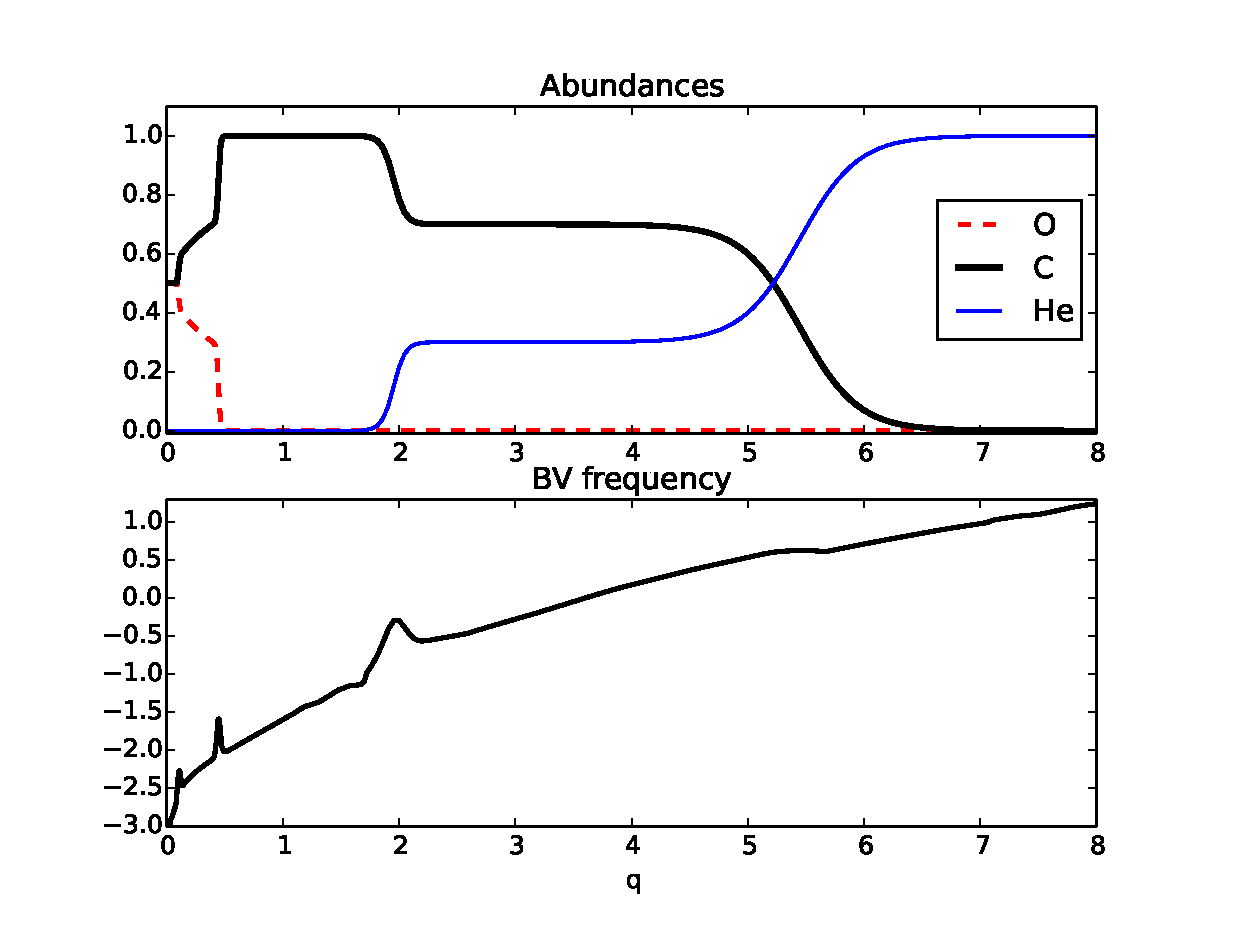
\includegraphics[width=1.0\columnwidth]{ffit1.eps}}
\epsscale{1.0}
 \plotone{ffit1.eps}
\caption{
{\em Upper panel:} Chemical composition profiles of the best fit model. The center of the model is 
to the left and the surface to the right.  $q=2$ corresponds to $M_r = 0.99 \: M_*$. The vertical axis
shows fractional abundances. 
{\em Lower panel:} The corresponding \bvf frequency ($\log{N^2}$ on the vertical axis). \label{ffit1}
}
\end{figure}

We started with a master grid (Table \ref{fitt1}) chosen so that it covered all relevant 
area of parameter space and had sufficient resolution to find any region of local minimum 
in the fitness parameter \citep{Bischoff-Kim11a,Bischoff-Kim14}. We used the maximum resolution 
that was computationally manageable. The master grid involved the computation 
of 10,483,200 models. We fit simultaneously all 15 periods, requiring all of them to be $\ell=1$ 
modes. A fitness map of this initial fit are shown in the left panel of Fig. \ref{ffit2}, and the 
parameters of the best fit model are listed in Table \ref{fitt1}.

\subsection{Asymptotic Period Spacing}
\label{periodspacing}

Before we refine the period-by-period fitting optimization, it is worthwhile to step back and consider 
what we can learn from the average period spacing of GD358. The average period spacing provides an 
asteroseismic measure of the mass and temperature of the star, independent of the details of 
internal chemical composition profiles. Higher $k$ modes are not strongly trapped in the core and 
according to asymptotic theory, they should be nearly evenly spaced in period. This spacing is 
given by \citet{Unno89}.

\begin{equation}
\label{fiteq2}
\Delta P = \frac{\pi}{\sqrt{\ell(\ell + 1)}}\left[\int_{r_1}^{r_2}\frac{N}{r}dr\right]^{-1},
\end{equation}

\noindent
where $r_1$ and $r_2$ are turning points of the mode and N is the Brunt-V\"{a}is\"{a}l\"{a} frequency. 
The asymptotic period spacing is $\ell$ dependent, with higher $\ell$ modes having smaller spacing. 
In the case of GD 358, we have a single $\ell=1$ sequence so we only need to worry about the dependence 
of the asymptotic period spacing on the \bvf frequency. Much if not all of GD 358's pulsation 
spectrum is close to the asymptotic limit, because the shortest period observed is a $k=8$ mode.

The dependence of $\Delta P$ on the \bvf frequency leads to higher mass and lower temperature models 
having a smaller period spacing (their interior is less compressible). This effect appears in asteroseismic 
fitting of white dwarfs and also sdB stars as a ubiquitous diagonal trend in contour maps of the quality 
of the fits in the mass-effective temperature plane \citep[e.g][]{Bischoff-Kim14,Castanheira09,Charpinet08}. 
One requirement for the periods of the model to match the observed periods is that the average period spacing 
in the models matches the average period spacing in the observed pulsation spectrum. If a good match occurs 
for a given mass and effective temperature, then models with lower mass but higher effective temperature 
will also match well.

We use the sequence of 13 consecutive $\ell=1$ modes found in GD358's pulsation spectrum to calibrate our models (Table~\ref{gd}). 
Using the $\ell=1$ sequence of modes, we compute an average period spacing of 39.08 seconds. We call 
this $\Delta P_{\rm obs}$. For each model in the master grid, we compute an asymptotic period spacing 
($\Delta P_{\rm calc}$). This asymptotic period spacing is calculated by first discarding the 10 lowest $k$ modes. 
The exact value of 10 is somewhat arbitrary, but it is chosen so that the modes we use in 
our computation are indeed in the asymptotic limit. The higher $k$ modes show weaker trapping than the 
lower $k$ modes. We then fit a line through the set ($k_i$,$P_i$). The slope gives us the asymptotic 
period spacing in the model. We also calculate the residuals of the fits and discard the models that have 
residuals above a certain limit. The limit is chosen by checking the procedure 
by eye on a few models. 

We show a contour map of the location of the models that best match the average period spacing of 
39.08 seconds in Fig. \ref{ffit2}, right panel. We place it side by side with a contour map showing 
the location of the best fit model in the same region of parameter space, based on the master grid 
fitting described in section \ref{grids}. Note how the best fit model falls right within the valley 
where the period spacings between GD358 and the models match. This should come as no surprise, as in 
order for 15 periods to fit reasonably well, the model period list should have a spacing similar to 
that of the observed period spectrum. The most recent spectroscopic determination of \citet{Koester2013} 
is far off the valley, at 24,000~K and $0.506^{+0.034}_{-0.051}$ \msun. Previous spectroscopic determinations, 
such as that of \citet{Bergeron2011}, do fall within the swath where the period spacings match.

%  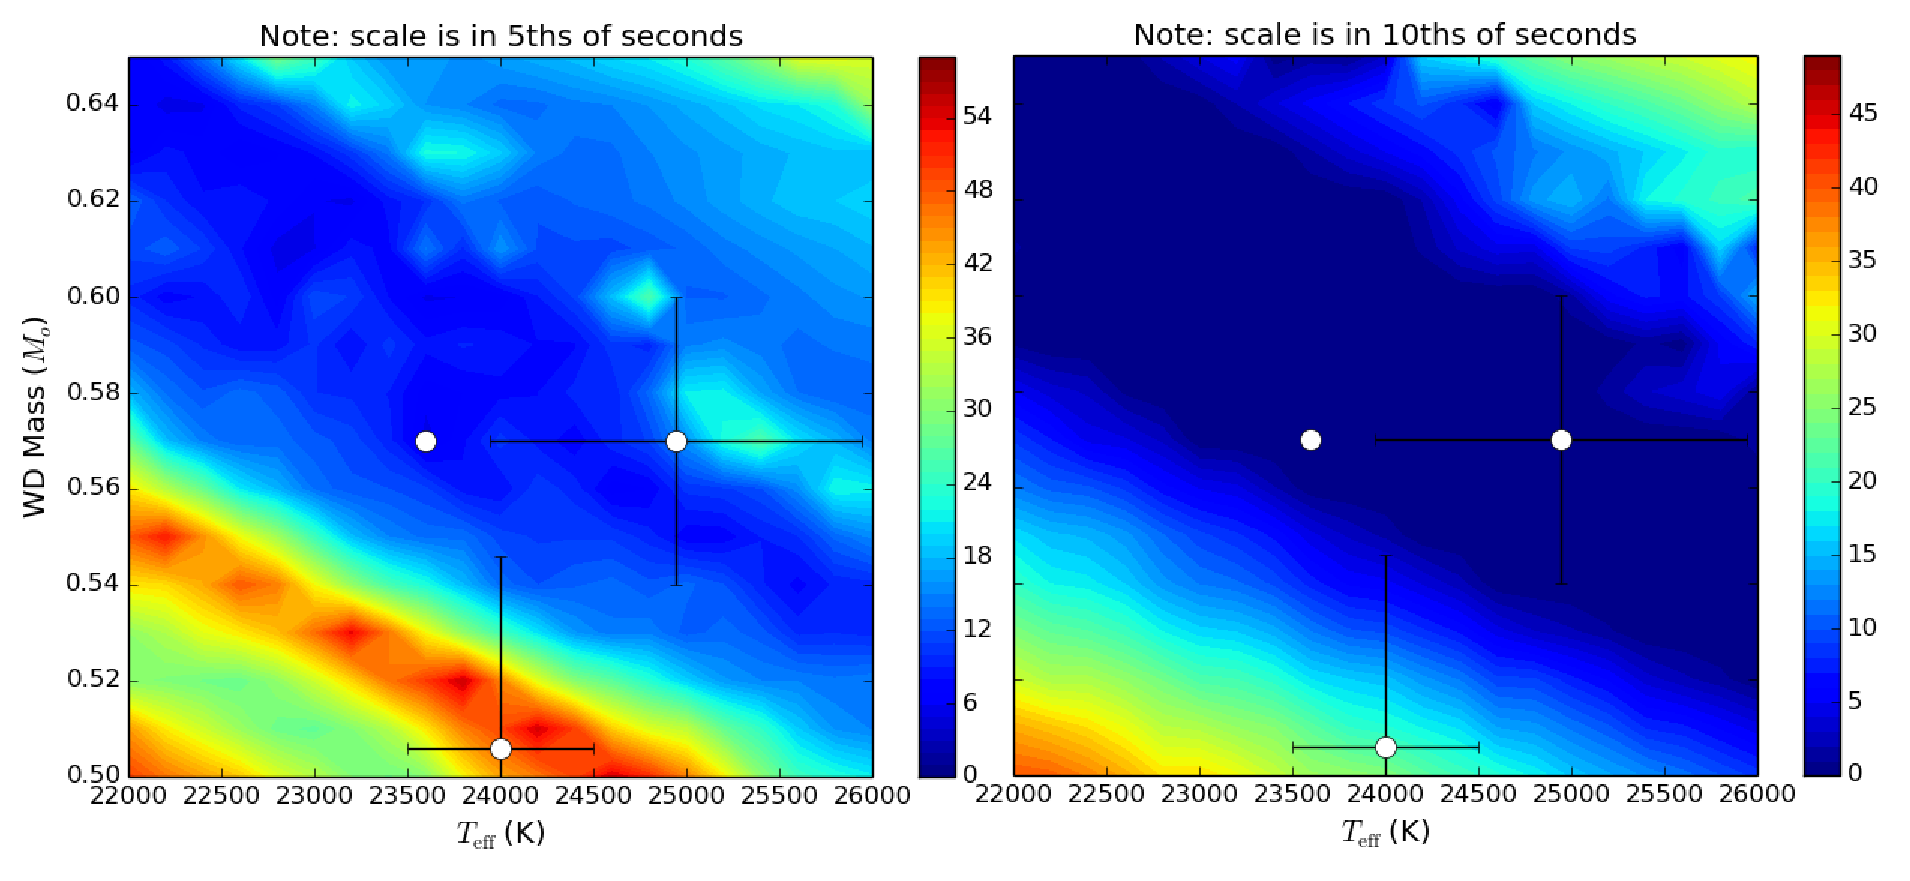
\includegraphics[width=1.0\columnwidth]{ffit2.eps}
\begin{figure}
\epsscale{1.0}
\plotone{ffit2.eps}
\caption{
{\it Left panel}: Contour map showing the location of the best fit models. The quantity plotted in 
the mass-effective temperature plane is the fitness parameter defined in equation \ref{fiteq1}. 
{\it Right panel}: Contour map of the difference between the average 
periods spacing determined from GD 358's periods and the asymptotic period spacing of the models, 
in the mass-effective temperature plane. The scale is in 10ths of seconds, so the worse matches 
pictured on the plot have $\left|\Delta P_{\rm obs}- \Delta P_{\rm calc}\right| \sim 5 \; \rm s$. 
We plotted the spectroscopic mass and temperature determinations of \citet{Bergeron2011} (higher mass), 
and that of \citet{Koester2013} (lower mass). The point without error bars corresponds to the 
best initial fit model. \label{ffit2}
}
\end{figure}

One can fit simultaneously the average period spacing and the individual periods 
formally while performing the fits by using some prescription to calculate the goodness of fit. 
This leads to a more complex relation than defined in equation \ref{fiteq1}. 
Note that the period spacing is a much weaker constraint than the individual period fit. 
If one takes 5.0 seconds as an upper limit for goodness of fit, that includes 4\% of the models in the 
period-by-period fit plot (left panel in Fig \ref{ffit2}), but the entire parameter plane 
for the average period spacing fit plot (right panel). In our refined fits, we limit ourselves to a 
region very near the best fit model found on the initial grid. This essentially limits our search 
to models that already match the average period spacing. We avoid sophisticated schemes to calculate 
the fitness parameter and simply use equation \ref{fiteq1}.


\subsection{Optimal Grid Resolution}
\label{refinedfits}


Having determined a more restricted region of parameter space to search for 
the best fit models, we now turn to the question of how fine we need to 
make our refined grid. We want to have a high enough resolution grid that 
we can be sure we captured a true minimum, but on the other hand, there are 
computational limitations to how many models we can afford to calculate, 
save, and process.

One way to gain a sense of how fine the grid needs to be is to make single 
parameter cuts through parameter space. Fig.  \ref{ffit3} shows such cuts 
for master grid models. The plot was made by fixing 5 of the 6 parameters 
to the best fit values of the best initial fit (see table \ref{fitt1}).
For some parameters, the fits seem to settle to a minimum in a 
smooth way, while for others, they exhibit jumps. For instance, the spike 
in the effective temperature plot at 27,800~K is due to a period (around 530~s) 
that goes away and then comes back. The model with the missing period fits poorly 
compared to the models on either side of it. The jump from \sigrms $\sim$ 5 s 
to \sigrms $\sim$ 30 s that happens from 28,400~K to 28,600~K is due to a discontinuous 
change in the period spectrum of the models. Namely, the appearance of a new mode 
between the 710 and 784~s modes of the 28,400~K model. 

\begin{figure}
\epsscale{1.0}
\plotone{ffit3.eps}
%  \includegraphics[scale=0.70,viewport=50 0 50 350]{f2.png}
%  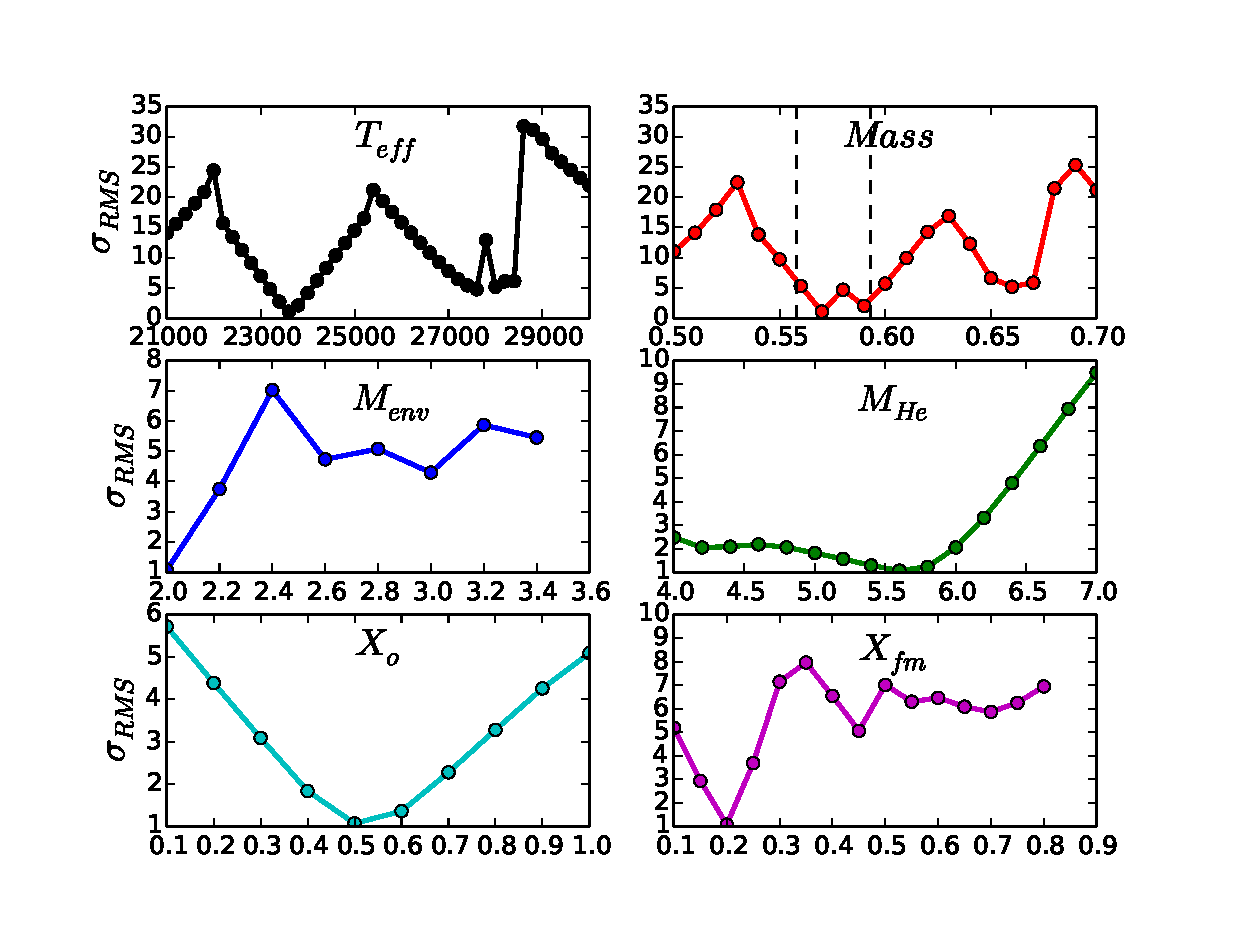
\includegraphics[width=0.9\columnwidth]{ffit3.eps}
\caption{
Dependence of the fitness parameter on different parameters. The 5 parameters other than the one shown 
on the horizontal axis in each plot are held to fixed values corresponding to the initial best fit
model (table \ref{ffit1}). The vertical dashed lines mark the ranges considered in the refined 
fitting. For the envelope mass, we went from \menv = -2.0 to -2.3.
 \label{ffit3}
}
\end{figure}

Discontinuities like these are unsettling, as it is easy to see that one might miss a best fit 
model if the grid is not fine enough. In order to quantify "fine enough", 
we ran systematic scans, computing models with 5 parameter fixed and allowing 
the 6th parameter to vary in very fine steps. We went down in 
step sizes to $\Delta {\rm T_{eff}}=1$~K, $\Delta M_*=0.0001 M_\odot$, 
$\Delta M_{\rm env}= \Delta M_{\rm He}=0.01$ dex, $\Delta X_o=0.01$, and $\Delta q_{\rm fm}=0.001$. 
Regardless of the behavior of individual modes in the models as the parameters vary, 
we can assert what step sizes will allow us to minimize our risk 
of missing a minimum, while minimizing the number of models to compute. We settled on step sizes of 
$\Delta {\rm T_{eff}}=50$~K, $\Delta M_*=0.0001 M_\odot$, $\Delta M_{\rm env}=\Delta M_{\rm He}=0.1$ dex,  
$\Delta X_o=0.1$, and $\Delta q_{\rm fm}=0.005$ for our refined grid.
		
\section{Results of the Period Fitting}
\label{results}

The parameters for our best fit model based on the refined grid are listed in Table \ref{fitt1} 
and the periods of that model in Table \ref{gd}. The goodness of fit of the model is \sigrms$=0.964$~s. 
We also list the Bayes Information Criterion (BIC) number, a statistic that
normalizes the quality of fits by number of free parameters and
number of constraints for comparison with other studies. For a discussion applied to this parameter
study, see \citet{Bischoff-Kim11a}. A negative BIC indicates a good quality of fit, given the number 
of constraints. One should keep in mind that the quality of fit is aided by the fact that some of 
the observed periods have large uncertainties.

In Fig. \ref{ffit4} we focus on the mass dependence of the fitness parameter to illustrate 
the effect a finer grid has on the fitting. We could have used less of a fine mesh in mass, 
but with our very fine mesh, we do get a better view of how the discontinuities first shown 
in Fig. \ref{ffit3} behave and that they are not true discontinuities, just large changes in 
goodness of fit for small changes in mass.

\begin{figure}
\epsscale{0.7}
\plotone{ffit4.eps}
%  \includegraphics[scale=0.70,viewport=50 0 50 350]{f2.png}
%  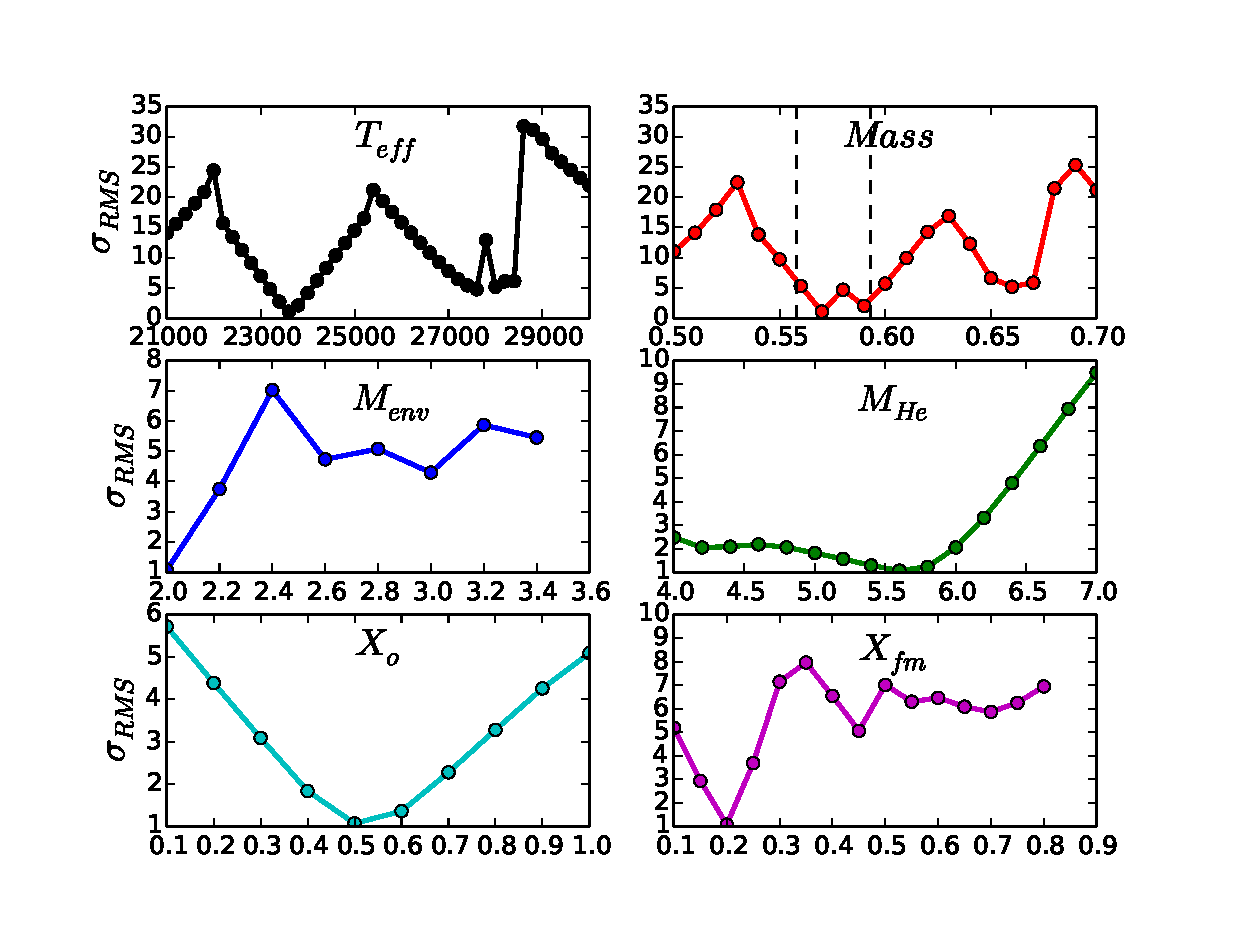
\includegraphics[width=0.9\columnwidth]{ffit3.eps}
\caption{
Dependence of the fitness parameter on mass alone based on 
the master grid of models (dashed line) and the refined mesh (solid line). \label{ffit4}
}
\end{figure}


Finally, we show the interior structure of the best fit model in Fig. \ref{ffit1}, with the corresponding \bvf frequency profile.

\subsection{Validation of the Fitting Method and Error Estimation}

With what we have discovered in section \ref{refinedfits}, it is only natural to be concerned about whether we have truly 
found a best fit. We performed a simple test to validate our fitting method, which consisted of using the exact same procedure 
to find a best fit to the periods of a model that was not on any of the grids we calculated, but that did have parameters that 
were very close to the best fit model. We used the period list for a model with parameters 
${\rm T_{eff}}=25630$~K, $M_*/M_\odot=0.57065$, \menv $=-2.05$ $M_{\rm He}=-5.55$, $X_o=0.52$, and $q_{\rm fm}=0.192$, 
including only the subset of 15 $\ell=1$ periods that match GD358's pulsation spectrum.

We first performed a fitting of the periods using the master (coarse) grid described in section \ref{grids}. This 
placed the best fit model in the appropriate region of parameter space. Then we refined our fits, using the grids 
described at the end of section \ref{periodspacing}. We are able to recover the best fit parameters adequately, with 
the all top 5 best fit models having parameters 
${\rm T_{eff}}=25000$~K, \mhe $=-2.1$, $M_{\rm env}=-5.5$, $X_o=0.50$, and $q_{\rm fm}=0.190$ and a 
mass ranging between  0.5730 and 0.5734 \msun. The best fit model has \sigrms $=0.31$~s. We remind t
he reader that the step sizes in the second phase of the fitting are 50~K for 
${\rm T_{eff}}$, 0.0001 \msun ~ for stellar mass, 0.1 dex for helium layer masses, 
0.1 for $X_o$, and 0.005 for $q_{\rm fm}$.

This test also allows us to place minimum error bars on at least some of the parameters found: $\pm 600$ ~ K in effective 
temperature, 0.05 and 0.02 dex on \menv and \mhe respectively, 0.02 on $X_o$, and 0.002 on $q_{\rm fm}$.


\section{Discussion and Conclusions}
\label{discussion}

We analyzed archival data and over a thousand hours of new observations on GD358, together covering a 
span of 33 years. With data spanning such a long period of time, we learn about the stability of the
different modes. We find that the shorter period modes tend to be more stable, while the longer period 
modes tend to vary more in frequency over time. \citet{Bell15} have observed and modeled such stochastic 
behavior in KIC 4552982, a red edge DAV observed nearly continuously for 1.5 years by \emph{Kepler}. 
In that star, the 361.58 s triplet has sharply defined peaks, while the rest of the modes, with much 
higher overtone numbers, are less stable. The stability of the low k modes is likely due to the fact 
that they are strongly trapped in the core. Unlike their higher k counterparts, they are affected very 
little by the convection zone near the surface.

In analyzing the data, we found 4 new modes, adding to the 11 modes known previously. With these 15 modes, 
we performed a new asteroseismic fit of GD358 with models that include carbon and oxygen core composition 
profiles based on the stellar evolution models of \citet{Salaris97}. We find a best fit effective temperature 
of 23,650~K and a mass of 0.5706 \msun ~ for GD358. While the temperature is close to the recent spectroscopic 
determination of 24000~K \citep{Koester2013}, the mass is over one sigma above the spectroscopic mass. On the 
other hand, the mass matches almost exactly that found by \citet{Bergeron2011} (but the effective 
temperature is low). The spectroscopic data point of \citet{Koester2013} is somewhat off the asymptotic 
period spacing trend (Fig. \ref{ffit2}, right panel).

In this study, we varied the parameters that have traditionally been varied in this type of 
asteroseismic fitting, so that we can place our results side by side with other studies of 
DBVs, including KIC 8626021 \citep{Bischoff-Kim14}, EC20058 \citep{Bischoff-Kim11a}, and 
CBS114 \citep{Metcalfe05a}. We now have 4 DBVs that were the object of asteroseismic fitting 
that used a consistent set of models. We find that cooler best fit models have thicker pure 
helium envelopes (Fig. \ref{ffit5}), in accordance with the outward diffusion of helium over time. 
To be consistent, we used the effective temperature found through the asteroseismic fitting of each 
star. Stellar mass also comes into play in diffusion. Ideally, we would like all 4 models to have 
the same mass. The models range in mass from 0.525 (EC20058) to 0.640 \msun ~ (CBS114). More detailed 
stellar evolution calculations would have to be performed in order to assess the significance of the 
trend observed with these 4 DBVs.

\begin{figure}
\epsscale{0.7}
\plotone{ffit5.eps}
%  \includegraphics[scale=0.70,viewport=50 0 50 350]{f2.png}
%  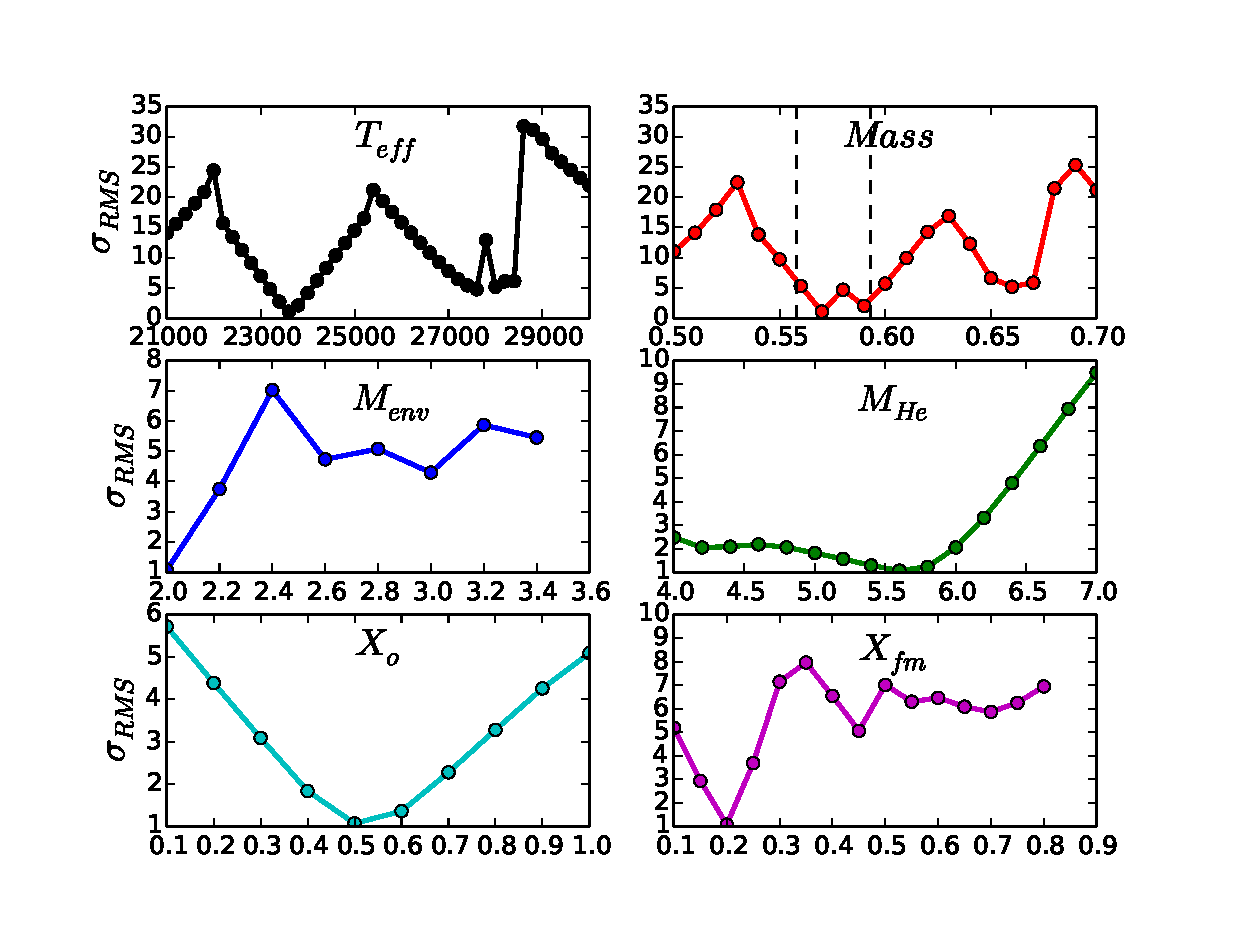
\includegraphics[width=0.9\columnwidth]{ffit3.eps}
\caption{
Relationship between effective temperature and pure helium layer mass in 4 DBVs fitted using similar 
models as GD358 in the present study. \label{ffit5}
}
\end{figure}

Numerical experiments of the type presented in section \ref{refinedfits} have shown that, consistent with 
the theory of non-radial oscillations, the shapes of the transition zones matter as much as where 
they occur \citep{Bischoff-Kim15}. Modern asteroseismic fitting vary parameters attached to the shape of 
transition zones \citep{Giammichele15}. We refrained from doing this in the present study because we wanted to 
compare our results with previous studies of DBVs. It is unclear how much of an effect on structure parameters a 
change in parameterization would have.

In fitting GD358, we discovered that two very close sets of parameters were able to yield very different fitness 
parameters. This is due to the fact that some periods can change values drastically for a small change in a given 
parameter. The periods tend to oscillate between two values and there remains a well defined minimum in parameter space, 
even if it is a double valued minimum. Any search algorithm that uses a small enough mesh should be able to find the 
minimum. This phenomenon likely became apparent while fitting GD358 because it is the first white dwarf for which 
we fit a long consecutive sequence of modes of the same $\ell$ with high resolution grids.

\acknowledgments


{\it Facilities:} \facility{MCAO:0.6m ()}, \facility{Struve()},
\facility{KPNO:2.1m ()}, 
\facility{}, \facility{BOAO:1.8m ()}, \facility{Lulin:1.8m ()},
\facility{Beijing:2.16m ()}, \facility{Maidanek:1.5m ()}, \facility{Peak Terskol}


\bibliographystyle{apj}
\bibliography{index_f}


\clearpage

\begin{deluxetable}{llrrr}
\tablecolumns{5}
\tabletypesize{\small}
\tablewidth{0pc}
\tablecaption{\label{journal}}
\tablehead{
\colhead{Run Name} & \colhead{Telescope} & \colhead{Detector} & \colhead{Date} & \colhead{Length}\\
\colhead{} & \colhead{} & \colhead{} & \colhead{} & \colhead{(hrs)}
}
\startdata
mcao070524-01 & MCAO 0.6 & CCD & 2007-05-24 & 4.0\\
mcao070531-02 & MCAO 0.6 & CCD & 2007-05-31 & 4.1\\
mcao080613-01 & MCAO 0.6 & CCD & 2008-06-13 & 2.0\\
mcao080617-02 & MCAO 0.6 & CCD & 2008-07-25 & 1.2\\
mcao080726-01 & MCAO 0.6 & CCD & 2008-07-26 & 1.7\\
mcao080730-01 & MCAO 0.6 & CCD & 2008-07-30 & 3.5\\
mcao080802-01 & MCAO 0.6 & CCD & 2008-08-02 & 3.7\\
pjmo080706-03 & PJMO 0.6 & CCD & 2008-07-06 & 5.1\\
suho080810-19 & Suhora 0.6 & CCD & 2008-08-10 & 4.7\\
suho080811-19 & Suhora 0.6 & CCD & 2008-08-11 & 2.5\\
boao090528-17 & BOAO 1.8 & CCD & 2009-05-28 & 2.0\\
kore090529-16 & BOAO 1.8 & CCD & 2009-05-29 & 2.4\\
mcao090513-01 & MCAO 0.6 & CCD & 2009-05-13 & 2.4\\
mcao090519-03 & MCAO 0.6 & CCD & 2009-05-19 & 3.2\\
mcao090520-01 & MCAO 0.6 & CCD & 2009-05-20 & 4.8\\
mcao090521-01 & MCAO 0.6 & CCD & 2009-05-21 & 4.9\\
mcao090522-01 & MCAO 0.6 & CCD & 2009-05-22 & 3.1\\
mcao090531-02 & MCAO 0.6 & CCD & 2009-05-31 & 2.1\\
mcao090601-01 & MCAO 0.6 & CCD & 2009-06-01 & 3.3\\
mole090526-20 & Moletai 1.65  & CCD & 2009-05-26 & 3.7\\
suho090520-19 & Suhora 0.6  & CCD & 2009-05-20 & 2.2\\
suho090521-19 & Suhora 0.6 & CCD & 2009-05-21 & 5.1\\
vien090525-19 & Vienna 0.6 & CCD & 2009-05-25 & 6.2\\
krak100523-20 & Krakow 0.4 & CCD & 2010-05-23 & 3.4\\
krak100526-20 & Krakow 0.4 & CCD & 2010-05-26 & 2.3\\
krak100616-20 & Krakow 0.4 & CCD & 2010-06-16 & 4.3\\
krak100617-20 & Krakow 0.4 & CCD & 2010-06-17 & 4.5\\
mcao100516-01 & MCAO 0.6 & CCD & 2010-05-16 & 2.0\\
mcao100521-01 & MCAO 0.6 & CCD & 2010-05-21 & 0.9\\
mcao100521-05 & MCAO 0.6 & CCD & 2010-05-21 & 0.8\\
mcao100526-01 & MCAO 0.6 & CCD & 2010-05-26 & 3.3\\
mcdo100517-06 & McDonald 2.1  & CCD & 2010-05-17 & 4.8\\
mole100516-22 & Moletai 1.65  & CCD & 2010-05-26 & 1.8\\
mole100517-22 & Moletai 1.65  & CCD & 2010-05-17 & 2.0\\
mole100520-21 & Moletai 1.65  & CCD & 2010-05-20 & 3.3\\
mole100521-21 & Moletai 1.65  & CCD & 2010-05-21 & 3.5\\
pjmo100519-04 & PJMO 0.6 & CCD & 2010-05-19 & 4.0\\
pjmo100520-02 & PJMO 0.6 & CCD & 2010-05-20 & 3.8\\
pjmo100521-05 & PJMO 0.6 & CCD & 2010-05-21 & 3.3\\
pjmo100522-02 & PJMO 0.6 & CCD & 2010-05-22 & 7.0\\
pjmo100523-04 & PJMO 0.6 & CCD & 2010-05-23 & 6.0\\
pjmo100524-02 & PJMO 0.6 & CCD & 2010-05-24 & 7.5\\
pjmo100527-02 & PJMO 0.6 & CCD & 2010-05-27 & 8.3\\
pjmo100528-02 & PJMO 0.6 & CCD & 2010-05-28 & 8.3\\
pjmo100619-03 & PJMO 0.6 & CCD & 2010-06-19 & 4.0\\
pjmo100622-02 & PJMO 0.6 & CCD & 2010-06-22 & 0.7\\
suho100617-21 & Suhora 0.6 & CCD & 2010-06-17 & 4.3\\
terb100516-17 & Terskol 2.0  & CCD & 2010-05-16 & 2.4\\
terb100520-17 & Terskol 2.0  & CCD & 2010-05-20 & 8.9\\
terb100521-20 & Terskol 2.0  & CCD & 2010-05-21 & 4.0\\
terb100524-19 & Terskol 2.0  & CCD & 2010-05-24 & 5.6\\
terb100525-17 & Terskol 2.0  & CCD & 2010-05-25 & 7.3\\
tueb100522-20 & Tuebingen 0.8 & SBig & 2010-05-22 & 5.9\\
tueb100523-20 & Tuebingen 0.8 & SBig & 2010-05-23 & 5.9\\
tueb100524-20 & Tuebingen 0.8 & SBig & 2010-05-24 & 6.0\\
tueb100604-20 & Tuebingen 0.8 & SBig & 2010-06-04 & 5.8\\
tueb100605-20 & Tuebingen 0.8 & SBig & 2010-06-05 & 5.3\\
turk100512-18 & Canakkale 1.2 & CCD & 2010-05-12 & 6.6\\
turk100513-22 & Canakkale 1.2 & CCD & 2010-05-13 & 2.8\\
turk100516-19 & Canakkale 1.2 & CCD & 2010-05-16 & 6.4\\
turk100520-19 & Canakkale 1.2 & CCD & 2010-05-20 & 1.1\\
turk100522-21 & Canakkale 1.2 & CCD & 2010-05-22 & 2.6\\
turk100523-19 & Canakkale 1.2 & CCD & 2010-05-23 & 6.0\\
turk100611-19 & Canakkale 1.2 & CCD & 2010-06-11 & 5.2\\
turk100613-19 & Canakkale 1.2 & CCD & 2010-06-13 & 5.3\\
turk100615-20 & Canakkale 1.2 & CCD & 2010-06-15 & 4.8\\
turk100618-19 & Canakkale 1.2 & CCD & 2010-06-18 & 4.5\\
turk100620-20 & Canakkale 1.2 & CCD & 2010-06-20 & 4.8\\
hvar110521-22 & Hvar 1.0 & CCD & 2011-05-21 & 2.6\\
hvar110526-19 & Hvar 1.0 & CCD & 2011-05-26 & 6.6\\
hvar110527-19 & Hvar 1.0 & CCD & 2011-05-27 & 3.5\\
hvar110529-19 & Hvar 1.0 & CCD & 2011-05-29 & 6.7\\
hvar110531-19 & Hvar 1.0 & CCD & 2011-05-31 & 4.3\\
hvar110602-19 & Hvar 1.0 & CCD & 2011-06-02 & 3.8\\
hvar110604-19 & Hvar 1.0 & CCD & 2011-06-04 & 6.6\\
hvar110606-20 & Hvar 1.0 & CCD & 2011-06-06 & 4.4\\
krak110506-20 & Krakow 0.4 & CCD & 2011-05-06 & 5.4\\
krak110509-19 & Krakow 0.4 & CCD & 2011-05-09 & 6.7\\
krak110510-19 & Krakow 0.4 & CCD & 2011-05-10 & 6.2\\
krak110511-19 & Krakow 0.4 & CCD & 2011-05-11 & 6.7\\
krak110512-19 & Krakow 0.4 & CCD & 2011-05-12 & 3.1\\
krak110516-19 & Krakow 0.4 & CCD & 2011-05-16 & 6.1\\
krak110517-19 & Krakow 0.4 & CCD & 2011-05-17 & 5.6\\
krak110518-19 & Krakow 0.4 & CCD & 2011-05-18 & 5.7\\
krak110519-20 & Krakow 0.4 & CCD & 2011-05-19 & 5.4\\
krak110520-20 & Krakow 0.4 & CCD & 2011-05-20 & 5.2\\
krak110522-21 & Krakow 0.4 & CCD & 2011-05-22 & 4.3\\
krak110523-23 & Krakow 0.4 & CCD & 2011-05-23 & 1.4\\
krak110524-19 & Krakow 0.4 & CCD & 2011-05-24 & 4.0\\
krak110525-20 & Krakow 0.4 & CCD & 2011-05-25 & 5.4\\
krak110526-20 & Krakow 0.4 & CCD & 2011-05-26 & 5.3\\
krak110529-20 & Krakow 0.4 & CCD & 2011-05-29 & 5.0\\
krak110530-20 & Krakow 0.4 & CCD & 2011-05-30 & 4.8\\
krak110531-20 & Krakow 0.4 & CCD & 2011-05-31 & 0.8\\
krak110604-20 & Krakow 0.4 & CCD & 2011-06-04 & 5.3\\
mole110426-22 & Moletai 1.65  & CCD & 2011-04-26 & 1.7\\
mole110427-21 & Moletai 1.65  & CCD & 2011-04-27 & 3.7\\
mole110430-20 & Moletai 1.65  & CCD & 2011-04-30 & 0.8\\
mole110502-20 & Moletai 1.65  & CCD & 2011-05-02 & 0.4\\
mole110502-21 & Moletai 1.65  & CCD & 2011-05-02 & 2.6\\
mole110505-20 & Moletai 1.65  & CCD & 2011-05-05 & 1.1\\
mole110510-21 & Moletai 1.65  & CCD & 2011-05-10 & 3.5\\
mtlm110426-05 & Mt. Lemmon 1.0 & CCD & 2011-04-26 & 6.3\\
mtlm110427-06 & Mt. Lemmon 1.0 & CCD & 2011-04-27 & 5.5\\
mtlm110428-04 & Mt. Lemmon 1.0 & CCD & 2011-04-28 & 7.1\\
mtlm110429-05 & Mt. Lemmon 1.0 & CCD & 2011-04-29 & 6.8\\
mtlm110430-05 & Mt. Lemmon 1.0 & CCD & 2011-04-30 & 6.4\\
mtlm110501-05 & Mt. Lemmon 1.0 & CCD & 2011-05-01 & 6.6\\
mtlm110502-05 & Mt. Lemmon 1.0 & CCD & 2011-05-02 & 6.5\\
naoc110426-13 & NAOC 0.5 & CCD & 2011-04-26 & 6.9\\
naoc110427-11 & NAOC 0.5 & CCD & 2011-04-27 & 3.3\\
naos110426-13 & NAOC 0.85 & CCD & 2011-04-26 & 6.9\\
naos110427-11 & NAOC 0.85 & CCD & 2011-04-27 & 3.3\\
naos110428-12 & NAOC 0.85 & CCD & 2011-04-28 & 2.6\\
naos110501-13 & NAOC 0.85 & CCD & 2011-05-01 & 7.1\\
naos110502-12 & NAOC 0.85 & CCD & 2011-05-02 & 8.3\\
naos110505-13 & NAOC 0.85 & CCD & 2011-05-05 & 7.0\\
pjmo110426-07 & PJMO 0.6 & CCD & 2011-04-26 & 3.0\\
pjmo110428-04 & PJMO 0.6 & CCD & 2011-04-28 & 2.0\\
pjmo110429-03 & PJMO 0.6 & CCD & 2011-04-29 & 2.5\\
pjmo110430-04 & PJMO 0.6 & CCD & 2011-04-30 & 3.0\\
pjmo110503-04 & PJMO 0.6 & CCD & 2011-05-03 & 2.6\\
pjmo110518-03 & PJMO 0.6 & CCD & 2011-05-18 & 6.7\\
pjmo110519-03 & PJMO 0.6 & CCD & 2011-05-19 & 2.7\\
pjmo110521-03 & PJMO 0.6 & CCD & 2011-05-21 & 2.7\\
pjmo110524-02 & PJMO 0.6 & CCD & 2011-05-24 & 5.2\\
pjmo110525-07 & PJMO 0.6 & CCD & 2011-05-25 & 3.2\\
pjmo110526-03 & PJMO 0.6 & CCD & 2011-05-26 & 7.0\\
pjmo110527-02 & PJMO 0.6 & CCD & 2011-05-27 & 0.8\\
pjmo110527-03 & PJMO 0.6 & CCD & 2011-05-27 & 6.7\\
suho110521-20 & Suhora 0.6 & CCD & 2011-05-21 & 5.2\\
suho110522-19 & Suhora 0.6 & CCD & 2011-05-22 & 5.9\\
suho110523-20 & Suhora 0.6 & CCD & 2011-05-23 & 5.6\\
suho110527-20 & Suhora 0.6 & CCD & 2011-05-27 & 2.0\\
suho110529-20 & Suhora 0.6 & CCD & 2011-05-29 & 4.6\\
suho110530-20 & Suhora 0.6 & CCD & 2011-05-30 & 4.9\\
terb110527-20 & Terskol 2.0  & CCD & 2011-05-27 & 2.4\\
terb110529-17 & Terskol 2.0  & CCD & 2011-05-27 & 4.4\\
terb110530-18 & Terskol 2.0  & CCD & 2011-05-30 & 2.6\\
terb110531-17 & Terskol 2.0  & CCD & 2011-05-31 & 1.8\\
terb110601-19 & Terskol 2.0  & CCD & 2011-06-01 & 3.3\\
tueb110504-19 & Tuebingen 0.8 & SBig & 2011-05-04 & 6.8\\
tueb110505-19 & Tuebingen 0.8 & SBig & 2011-05-05 & 6.8\\
tueb110506-19 & Tuebingen 0.8 & SBig & 2011-05-06 & 6.7\\
tueb110508-19 & Tuebingen 0.8 & SBig & 2011-05-08 & 6.6\\
tueb110509-19 & Tuebingen 0.8 & SBig & 2011-05-09 & 6.7\\
tueb110513-19 & Tuebingen 0.8 & SBig & 2011-05-13 & 2.2\\
tueb110518-22 & Tuebingen 0.8 & SBig & 2011-05-18 & 4.1\\
tueb110523-20 & Tuebingen 0.8 & SBig & 2011-05-23 & 5.9\\
tueb110524-20 & Tuebingen 0.8 & SBig & 2011-05-24 & 5.9\\
tueb110525-20 & Tuebingen 0.8 & SBig & 2011-05-24 & 6.0\\
tueb110529-20 & Tuebingen 0.8 & SBig & 2011-05-29 & 5.9\\
tueb110530-20 & Tuebingen 0.8 & SBig & 2011-05-30 & 3.4\\
tubi110602-00 & Tubitak 1.0  & CCD & 2011-06-02 & 1.1\\
tubi110602-23 & Tubitak 1.0  & CCD & 2011-06-02 & 2.0\\
tubi110603-20 & Tubitak 1.0  & CCD & 2011-06-03 & 5.2\\
boao120418-18 & BOAO 1.8 & CCD & 2012-04-18 & 1.7\\
krak120418-00 & Krakow 0.4 & CCD & 2012-04-18 & 1.8\\
krak120421-00 & Krakow 0.4 & CCD & 2012-04-21 & 4.6\\
krak120423-00 & Krakow 0.4 & CCD & 2012-04-23 & 1.7\\
krak120428-00 & Krakow 0.4 & CCD & 2012-04-28 & 6.6\\
krak120429-00 & Krakow 0.4 & CCD & 2012-04-29 & 6.1\\
krak120430-00 & Krakow 0.4 & CCD & 2012-04-30 & 6.7\\
mtlm120419-10 & Mt. Lemmon 1.0 & CCD & 2012-04-19 & 1.7\\
mtlm120420-10 & Mt. Lemmon 1.0 & CCD & 2012-04-20 & 1.4\\
mtlm120421-05 & Mt. Lemmon 1.0 & CCD & 2012-04-21 & 6.2\\
mtlm120422-07 & Mt. Lemmon 1.0 & CCD & 2012-04-22 & 4.8\\
na50120524-12 & NAOC 0.5 & CCD & 2012-05-24 & 4.5\\
na50120525-12 & NAOC 0.5 & CCD & 2012-05-25 & 4.4\\
na50120526-14 & NAOC 0.5 & CCD & 2012-05-26 & 3.3\\
na50120527-12 & NAOC 0.5 & CCD & 2012-05-27 & 4.9\\
na50120530-13 & NAOC 0.5 & CCD & 2012-05-30 & 6.0\\
pjmo120425-03 & PJMO 0.6 & CCD & 2012-04-25 & 7.2\\
pjmo120426-03 & PJMO 0.6 & CCD & 2012-04-26 & 4.3\\
prom120430-04 & PROMPT 0.4 & CCD & 2012-04-30 & 2.2\\
prom120430-07 & PROMPT 0.4 & CCD & 2012-04-30 & 1.1\\
prom120501-04 & PROMPT 0.4 & CCD & 2012-05-01 & 4.5\\
prom120502-04 & PROMPT 0.4 & CCD & 2012-05-02 & 4.4\\
prom120503-04 & PROMPT 0.4 & CCD & 2012-05-03 & 0.9\\
prom120504-04 & PROMPT 0.4 & CCD & 2012-05-04 & 4.5\\
prom120509-04 & PROMPT 0.4 & CCD & 2012-05-09 & 4.3\\
prom120510-04 & PROMPT 0.4 & CCD & 2012-05-10 & 4.1\\
prom120511-03 & PROMPT 0.4 & CCD & 2012-05-11 & 4.1\\
prom120512-03 & PROMPT 0.4 & CCD & 2012-05-12 & 4.0\\
prom120513-03 & PROMPT 0.4 & CCD & 2012-05-13 & 2.1\\
prom120514-03 & PROMPT 0.4 & CCD & 2012-05-14 & 4.0\\
prom120515-03 & PROMPT 0.4 & CCD & 2012-05-15 & 4.0\\
suho120501-20 & Suhora 0.6 & CCD & 2012-05-01 & 6.0\\
suho120502-21 & Suhora 0.6 & CCD & 2012-05-02 & 5.1\\
suho120503-23 & Suhora 0.6 & CCD & 2012-05-03 & 2.4\\
suho120505-19 & Suhora 0.6 & CCD & 2012-05-05 & 2.1\\
tubi120420-01 & Tubitak 1.0  & CCD & 2012-04-20 & 1.0\\
tubi120423-19 & Tubitak 1.0  & CCD & 2012-04-23 & 6.6\\
tubi120512-20 & Tubitak 1.0  & CCD & 2012-04-23 & 5.2\\
caam130412-21 & Cannakkale 1.2 & CCD & 2013-04-12 & 4.0\\
caam130417-21 & Cannakkale 1.2 & CCD & 2013-04-17 & 3.2\\
caam130418-21 & Cannakkale 1.2 & CCD & 2013-04-18 & 4.5\\
krak130418-00 & Krakow 0.4 & CCD & 2013-04-18 & 6.7\\
krak130421-00 & Krakow 0.4 & CCD & 2013-04-18 & 7.4\\
krak130425-00 & Krakow 0.4 & CCD & 2013-04-25 & 6.7\\
krak130426-00 & Krakow 0.4 & CCD & 2013-04-26 & 2.1\\
naos130503-13 & NAOC 0.85 & CCD & 2013-05-03 & 6.0\\
pjmo130429-06 & PJMO 0.6 & CCD & 2013-04-29 & 2.7\\
pjmo130430-07 & PJMO 0.6 & CCD & 2013-04-30 & 2.1\\
pjmo130503-07 & PJMO 0.6 & CCD & 2013-05-03 & 3.6\\
pjmo130505-04 & PJMO 0.6 & CCD & 2013-05-05 & 6.8\\
suho130422-21 & Suhora 0.6 & CCD & 2013-04-22 & 4.6\\
suho130425-20 & Suhora 0.6 & CCD & 2013-04-25 & 5.9\\
suho130426-20 & Suhora 0.6 & CCD & 2013-04-26 & 5.4\\
suho130501-19 & Suhora 0.6 & CCD & 2013-05-01 & 6.1\\
suho130504-21 & Suhora 0.6 & CCD & 2013-05-04 & 4.4\\
suho130505-19 & Suhora 0.6 & CCD & 2013-05-05 & 5.5\\
caam140610-19 & Cannakkale 1.2 & CCD & 2014-046-10 & 5.5\\
krak140530-21 & Krakow 0.4 & CCD & 2014-05-30 & 2.4\\
krak140604-20 & Krakow 0.4 & CCD & 2014-06-04 & 5.5\\
krak140606-20 & Krakow 0.4 & CCD & 2014-06-06 & 4.7\\
krak140607-20 & Krakow 0.4 & CCD & 2014-06-07 & 5.1\\
krak140608-20 & Krakow 0.4 & CCD & 2014-06-08 & 5.2\\
krak140609-19 & Krakow 0.4 & CCD & 2014-06-09 & 4.7\\
krak140610-20 & Krakow 0.4 & CCD & 2014-06-10 & 2.4\\
mcao140602-05 & MCAO 0.6 & CCD & 2014-06-02 & 3.0\\
mcao140603-01 & MCAO 0.6 & CCD & 2014-06-03 & 4.1\\
mcao140607-01 & MCAO 0.6 & CCD & 2014-06-07 & 4.0\\
mcao140608-01 & MCAO 0.6 & CCD & 2014-06-08 & 3.9\\
mole140526-20 & Moletai 1.65  & CCD & 2014-05-26 & 2.5\\
mole140527-20 & Moletai 1.65  & CCD & 2014-05-27 & 3.7\\
mole140605-20 & Moletai 1.65  & CCD & 2014-06-05 & 3.3\\
mole140607-20 & Moletai 1.65  & CCD & 2014-06-07 & 2.9\\
naos140605-15 & NAOC 0.85 & CCD & 2014-06-05 & 5.7\\
naos140606-17 & NAOC 0.85 & CCD & 2014-06-06 & 3.9\\
pjmo140519-04 & PJMO 0.6 & CCD & 2014-05-19 & 4.0\\
pjmo140529-03 & PJMO 0.6 & CCD & 2014-05-29 & 5.4\\
pjmo140530-03 & PJMO 0.6 & CCD & 2014-05-30 & 4.3\\
pjmo140531-02 & PJMO 0.6 & CCD & 2014-05-31 & 5.0\\
pjmo140601-03 & PJMO 0.6 & CCD & 2014-06-01 & 3.3\\
pjmo140602-02 & PJMO 0.6 & CCD & 2014-06-02 & 4.5\\
pjmo140603-02 & PJMO 0.6 & CCD & 2014-06-03 & 7.1\\
pjmo140604-04 & PJMO 0.6 & CCD & 2014-06-04 & 5.8\\
pjmo140611-03 & PJMO 0.6 & CCD & 2014-06-11 & 5.9\\
suho140604-19 & Suhora 0.6 & CCD & 2014-06-04 & 4.4\\
suho140606-20 & Suhora 0.6 & CCD & 2014-06-06 & 4.7\\
ters140604-20 & Terskol 0.6  & CCD & 2014-06-04 & 2.0\\
ters140619-20 & Terskol 0.6  & CCD & 2014-06-19 & 6.0\\
tsao140524-17 & Tien Shan 1.0 & CCD & 2014-05-24 & 4.7\\
tsao140525-16 & Tien Shan 1.0 & CCD & 2014-05-25 & 6.0\\
tsao140610-15 & Tien Shan 1.0 & CCD & 2014-06-10 & 1.0\\
tsao140611-16 & Tien Shan 1.0 & CCD & 2014-06-11 & 6.0\\
tsao140613-17 & Tien Shan 1.0 & CCD & 2014-06-13 & 4.6\\
tsao140616-19 & Tien Shan 1.0 & CCD & 2014-06-16 & 1.4\\
tsao140619-17 & Tien Shan 1.0 & CCD & 2014-06-19 & 4.8\\
tsao140620-18 & Tien Shan 1.0 & CCD & 2014-06-20 & 3.1\\
tsao140627-16 & Tien Shan 1.0 & CCD & 2014-06-27 & 5.9\\
tsao140628-16 & Tien Shan 1.0 & CCD & 2014-06-28 & 5.9\\
krak150420-20 & Krakow 0.4 & CCD & 2015-05-20 & 2.1\\
krak150421-19 & Krakow 0.4 & CCD & 2015-05-21 & 7.5\\
pjmo150420-03 & PJMO 0.6 & CCD & 2015-04-20 & 7.3\\
pjmo150421-05 & PJMO 0.6 & CCD & 2015-04-21 & 5.4\\
pjmo150422-03 & PJMO 0.6 & CCD & 2015-04-22 &4.7\\
pjmo150426-03 & PJMO 0.6 & CCD & 2015-04-26 &7.4\\
prom150428-08 & PROMPT 0.4 & CCD & 2015-04-28 &6.5\\
prom150429-03 & PROMPT 0.4 & CCD & 2015-04-29 & 6.6\\
prom150501-03 & PROMPT 0.4 & CCD & 2015-05-01 & 6.2\\
mcao160710-01 & MCAO 0.6 & CCD & 2016-07-10 & 2.0\\
mcao160711-01 & MCAO 0.6 & CCD & 2016-07-11 & 1.5\\
mcao160711-03 & MCAO 0.6 & CCD & 2016-07-11 & 2.0\\
mcao160712-01 & MCAO 0.6 & CCD & 2016-07-12 & 1.2\\
mcao160718-01 & MCAO 0.6 & CCD & 2016-07-18 & 1.2\\
mcao160721-03 & MCAO 0.6 & CCD & 2016-07-21 & 2.0\\
mcao160805-02 & MCAO 0.6 & CCD & 2016-08-05 & 1.2\\
pjmo160802-03 & PJMO 0.6 & CCD & 2016-08-02 & 4.6\\ 
pjmo160804-02 & PJMO 0.6 & CCD & 2016-08-04 & 5.7\\
pjmo160805-02 & PJMO 0.6 & CCD & 2016-08-05 & 5.6\\
pjmo160806-02 & PJMO 0.6 & CCD & 2016-08-06 & 6.0\\
pjmo160808-03 & PJMO 0.6 & CCD & 2016-08-08 & 4.8\\ 
suho160723-19 & Suhora 0.6 & CCD & 2016-07-23 & 5.5\\
tueb160716-21 & Tuebingen 0.8 & CCD & 2016-07-16 & 2.0\\
tueb160718-20 & Tuebingen 0.8 & CCD & 2016-07-18 & 4.5\\
tueb160719-20 & Tuebingen 0.8 & CCD & 2016-07-19 & 6.0\\
tueb160729-22 & Tuebingen 0.8 & CCD & 2016-07-29 & 4.2\\
tueb160730-20 & Tuebingen 0.8 & CCD & 2016-07-30 & 4.0\\
tueb160801-20 & Tuebingen 0.8 & CCD & 2016-08-01 & 2.6\\
tueb160803-20 & Tuebingen 0.8 & CCD & 2016-08-03 & 2.5\\
tueb160807-20 & Tuebingen 0.8 & CCD & 2016-08-07 & 4.9\\
warw160802-20 & Warwick 1.0m & CCD & 2016-08-02 & 5.0\\
warw160803-20 & Warwick 1.0m & CCD & 2016-08-03 & 4.6\\
warw160804-20 & Warwick 1.0m & CCD & 2016-08-04 & 5.0\\

\enddata
\tablecomments{Data from the Warwick 1.0m telescope was obtained during an engineering run.}
\end{deluxetable}

\clearpage

\begin{deluxetable}{llllr}
\tablecolumns{4}
\tablewidth{0pc}
\tablecaption{1982-2006 Detected Independent Frequencies
\label{freq1}
}
\tablehead{
\colhead{Frequency} &  \colhead{Period} & \colhead{Amplitude} &  \colhead{Signal/Noise}   &\\
\colhead{\muHz} & \colhead{s} & \colhead{mma} & \colhead{}
}
\startdata

1982 & & & \\
& & & & \\
$1236.483\pm0.07$ & 808.75 & $16.70\pm0.06$ & 9.4\\
$1431.112\pm0.04$ & 698.76 & $30.86\pm0.06$ & 11.4\\
$1613.842\pm0.05$ & 619.65 & $26.12\pm0.06$ & 9.7\\
$1618.845\pm0.06$ & 617.72 & $29.34\pm0.06$ & 10.9\\
$2368.563\pm0.10$ & 422.20 & $12.52\pm0.06$ & 5.8\\
\\
1984 & & & \\
\\
$1124.701\pm3.5$ & 889.13 & $24.7\pm1.1$  & 7.2\\
$1626.474\pm3.5$ & 614.83 & $25.9\pm1.1$ & 6.8\\
\\
1985 & & & \\
\\
$1166.944\pm0.05$ & 856.94 & $6.43\pm0.06$ & 11\\           
$1176.489\pm0.03$ & 849.99 & $35.70\pm0.06$ & 16.0\\
$1614.554\pm0.04$ & 619.37 & $9.15\pm0.06$ & 4.6\\
$2351.762\pm0.04$ & 425.22 & $14.34\pm0.06$ & 12\\
\\
1986 & & & \\
\\
$1081.025\pm0.03$ & 925.05 & $5.1\pm0.4$ & 4.6\\
$1160.678\pm0.03$ & 861.57 & $4.9\pm0.4$ & 4.5  \\
$1223.803\pm0.02$ & 817.12 & $9.3\pm0.4$ & 9.1  \\
$1233.585\pm0.01$ & 810.65 & $14.9\pm0.4$ & 14.5\\
$1385.240\pm0.03$ & 721.90 & $6.7\pm0.4$ & 6.4  \\
$1426.181\pm0.01$ & 701.17 & $14.2\pm0.4$ & 14.3\\
$1525.030\pm0.01$ & 655.72 & $21.3\pm0.4$ & 21.4\\
$1611.691\pm0.01$ & 620.47 & $20.9\pm0.4$ & 20.9\\
$2157.783\pm0.04$ & 463.44 & $2.4\pm0.4$ & 4  \\  
$2165.564\pm0.03$ & 461.77 & $4.8\pm0.4$ & 4\\
$2368.938\pm0.03$ & 422.13 & $5.8\pm0.4$ & 5.6\\
\\
1990 & & & \\
\\
$1112.933\pm0.03$ & 898.53 & $2.31\pm0.32$ & 4.0\\
$1114.180\pm0.03$ & 897.52 & $2.44\pm0.32$ & 4.1\\
$1118.324\pm0.02$ & 894.20 & $5.24\pm0.32$ & 8.9  \\      
$1119.089\pm0.03$ & 893.58 & $2.83\pm0.32$  & 4.8\\
$1224.216\pm0.03$ & 816.83 & $22.17\pm0.32$  & 4.0 \\       
$1233.413\pm0.03$ & 810.76 & $4.80\pm0.32$   & 8.4\\
$1245.395\pm0.03$ & 802.96 & $2.17 \pm0.32$  & 4.0  \\      
$1288.995\pm0.03$ & 775.80 & $3.50\pm0.32$   & 6.3\\
$1291.229\pm0.03$ & 774.46 & $4.31\pm0.32$   & 7.6  \\      
$1295.400\pm0.03$ & 771.96 & $3.27 \pm0.32$  & 5.8\\
$1297.540\pm0.01$ & 770.69 & $14.76\pm0.32$  & 26.1\\
$1304.075\pm0.03$ & 766.83 & $4.67\pm0.32$   & 8.3\\
$1355.447\pm0.03$ & 737.76 & $2.20\pm0.32$   & 4.0  \\      
$1361.728\pm0.03$ & 734.36 & $2.90\pm0.32$   & 5.2\\
$1368.588\pm0.03$ & 730.68 & $3.32\pm0.32$   & 5.9  \\      
$1375.434\pm0.03$ & 727.04 & $3.18\pm0.32$   & 5.7\\
$1421.041\pm0.02$ & 703.71 & $8.22\pm0.32$   & 15.1\\
$1423.704\pm0.03$ & 702.39 & $3.11\pm0.32$   & 5.8\\
$1427.365\pm0.01$ & 700.59 & $19.39\pm0.32$  & 35.8\\
$1428.663\pm0.03$ & 699.96 & $2.61 \pm0.32$  & 4.8\\
$1433.729\pm0.02$ & 697.48 & $7.29\pm0.32$   & 13.5 \\      
$1435.209\pm0.03$ & 696.76 & $3.50\pm0.32$   & 6.5\\
$1512.798\pm0.02$ & 661.03 & $5.57\pm0.32$   & 10.7  \\     
$1518.661\pm0.02$ & 658.47 & $8.34\pm0.32$   & 15.9\\
$1519.372\pm0.02$ & 658.17 & $5.88\pm0.32$   & 11.2  \\     
$1524.924\pm0.02$ & 655.77 & $5.98\pm0.32$   & 11.2\\
$1525.498\pm0.02$ & 655.52 & $6.95\pm0.32$   & 13.0  \\     
$1611.741\pm0.02$ & 620.45 & $6.09\pm0.32$   & 12.3\\
$1617.380\pm0.03$ & 618.28 & $4.69\pm0.32$   & 9.7   \\     
$1623.709\pm0.02$ & 615.87 & $5.04\pm0.32$   & 10.2\\
$2154.009\pm0.03$ & 464.25 & $4.40\pm0.32$   & 11.2 \\      
$2157.765\pm0.03$ & 463.44 & $2.27\pm0.32$   & 5.8\\
$2358.946\pm0.02$ & 423.92 & $5.63\pm0.32$   & 14.1  \\     
$2362.507\pm0.02$ & 423.28 & $5.71\pm0.32$   & 14.3\\
$2366.408\pm0.03$ & 422.58 & $4.59\pm0.32$   & 11.5\\
\\
1991 & & & \\
\\
$1296.087\pm0.13$ & 771.55 & $10.11\pm0.41$ & 17.7\\
$1296.577\pm0.13$ & 771.26 & $18.25\pm0.41$ & 29.8\\
$1308.777\pm0.05$ & 764.07 & $5.02\pm0.41$ & 9.9\\
$1396.945\pm0.05$ & 715.85 & $3.95\pm0.41$ & 8.4\\
$1419.934\pm0.01$ & 704.26 & $29.3\pm0.41$ & 45.6\\
$1423.333\pm0.04$ & 702.58 & $5.23\pm0.41$ & 6.3\\
$1427.062\pm0.04$ & 700.74 & $5.02\pm0.41$ & 7.4\\
$1443.381\pm0.05$ & 692.82 & $4.81\pm0.41$ & 9.7\\
$2150.307\pm0.05$ & 465.05 & $2.36\pm0.41$ & 4.1\\
$2154.389\pm0.05$ & 464.17 & $2.79\pm0.41$ & 4.6\\
$2157.939\pm0.05$ & 463.41 & $2.62\pm0.41$ & 4.4\\
$2370.121\pm0.04$ & 421.92 & $5.01\pm0.41$ & 9.2\\
$2374.211\pm0.05$ & 421.19 & $3.26\pm0.41$ & 5.7\\
$2378.195\pm0.04$ & 420.49 & $5.58\pm0.41$ & 10.7\\
\\
1992 & & & \\
\\
$1035.357\pm0.05$ & 965.85 & $7.35\pm0.31$ & 4.1\\
$1101.952\pm0.05$ & 907.48 & $6.40\pm0.31$ & 3.7\\
$1195.349\pm0.003$ & 836.58 & $6.90\pm0.31$ & 4.1\\
$1233.263\pm0.001$ & 810.86 & $20.79\pm0.31$ & 13.5\\
$1242.854\pm0.003$ & 804.60 & $14.20\pm0.31$ & 8.8\\
$1265.279\pm0.003$ & 790.34 & $12.25\pm0.31$ & 7.1\\
$1420.845\pm0.001$ & 703.81 & $20.59\pm0.31$& 13.1\\
$1438.411\pm0.003$ & 695.21 & $17.71\pm0.31$ & 11.9\\
$1622.795\pm0.003$ & 616.22 & $14.26\pm0.31$ & 9.2\\
$1628.812\pm0.004$ & 613.94 & $10.9\pm0.31$7 & 6.5\\
$2162.104\pm0.007$ & 462.51 & $4.26\pm0.31$ & 4.2\\
$2166.094\pm0.007$ & 461.66 & $5.66\pm0.31$ & 4.8\\
$2351.041\pm0.007$ & 425.34 & $6.75\pm0.31$ & 5.2\\
$2359.162\pm0.007$ & 423.88 & $6.55\pm0.31$& 9.2\\\
$2366.443\pm0.007$ & 422.58 & $7.17\pm0.31$ & 6.3\\
\\
1994 & & & \\
\\
$939.264\pm0.007$ & 1064.66 & $2.36\pm0.10$ & 5.7\\
$1024.773\pm0.011$ & 975.83 & $3.46\pm0.10$ & 8.8\\
$1064.931\pm0.012$ & 939.03 & $2.82\pm0.10$ & 7.4\\
$1106.833\pm0.013$ & 903.48 & $2.56\pm0.10$ & 7.0\\
$1113.548\pm0.012$ & 898.03 & $3.95\pm0.10$ & 9.4\\
$1164.637\pm0.012$ & 858.64 & $3.12\pm0.10$ & 8.6\\
$1176.684\pm0.013$ & 849.85 & $2.79\pm0.10$ & 7.2\\
$1224.306\pm0.012$ & 816.79 & $3.28\pm0.10$ & 9.1\\
$1234.488\pm0.013$ & 810.05 & $2.70\pm0.10$ & 7.7\\
$1235.491\pm0.005$ & 809.39 & $13.13\pm0.10$ & 37.3\\
$1242.357\pm0.013$ & 804.92 & $3.33\pm0.10$ & 9.1\\
$1246.494\pm0.013$ & 802.25 & $2.69\pm0.10$ & 7.8\\
$1286.550\pm0.003$ & 777.27 & $9.45\pm0.10$ & 27.6\\
$1291.023\pm0.009$ & 774.58 & $6.07\pm0.10$& 17.8\\
$1293.244\pm0.009$ & 773.25 & $5.85\pm0.10$ & 16.1\\
$1297.737\pm0.005$ & 770.57 & $21.5\pm0.10$ & 61.9\\
$1298.710\pm0.010$ & 769.99 & $4.45\pm0.10$ & 12.5\\
$1304.464\pm0.009$ & 766.64 & $6.84\pm0.10$ & 19.9\\ 
$1305.352\pm0.013$ & 766.08 & $2.54\pm0.10$ & 7.0\\
$1309.003\pm0.013$ & 763.94 & $2.76\pm0.10$ & 8.4\\
$1312.045\pm0.013$ & 762.17 & $2.67\pm0.10$ & 7.9\\
$1419.641\pm0.003$ & 704.40 & $18.70\pm0.10$ & 54.4\\
$1422.947\pm0.013$ & 702.77 & $2.86\pm0.10$ & 8.2\\
$1426.395\pm0.003$ & 701.07 & $16.05\pm0.10$ & 46.6\\
$1430.851\pm0.005$ & 698.88 & $10.35\pm0.10$ & 30.1\\
$1433.167\pm0.010$ & 697.75 & $4.06\pm0.10$ & 11.6\\
$1437.607\pm0.006$ & 695.60 & $8.28\pm0.10$ & 24.1\\
$1438.523\pm0.011$ & 695.16 & $3.68\pm0.10$ & 10.7\\
$1440.997\pm0.012$ & 693.96 & $2.48\pm0.10$ & 7.2\\
$1441.910\pm0.009$ & 693.52 & $4.09\pm0.10$ & 11.9\\
$1611.351\pm0.009$ & 620.60 & $5.12\pm0.10$ & 14.2\\
$1617.450\pm0.010$ & 618.26 & $3.61\pm0.10$ & 9.5\\
$1618.545\pm0.009$ & 617.84 & $4.04\pm0.10$ & 11.2\\
$1624.624\pm0.009$ & 615.53 & $5.83\pm0.10$ & 16.1\\
$1625.634\pm0.009$ & 615.14 & $4.89\pm0.10$ & 13.9\\
$2150.498\pm0.010$ & 465.01 & $3.22\pm0.10$ & 9.4\\
$2154.130\pm0.010$ & 464.22 & $4.75\pm0.10$ & 13.7\\
$2157.844\pm0.012$ & 463.43 & $2.70\pm0.10$ & 7.6\\
$2358.880\pm0.010$ & 423.93 & $4.53\pm0.10$ & 13.5\\
$2362.636\pm0.005$ & 423.26 & $9.29\pm0.10$ & 31.2\\
$2366.505\pm0.011$ & 422.56 & $4.26\pm0.10$ & 13.2\\
\\
1996 & & & \\
\\
$937.695\pm0.028$ & 1066.44 & $4.27\pm0.28$ & 3.5\\
$1024.276\pm0.028$ & 976.30 & $6.78\pm0.28$ & 6.4\\
$1104.483\pm0.025$ & 905.40 & $5.55\pm0.28$ & 5.1\\
$1178.461\pm0.025$ & 848.56 & $5.34\pm0.28$ & 5.5\\
$1227.936\pm0.022$ & 814.37 & $7.66\pm0.28$ & 7.5\\
$1233.14\pm0.015$  & 810.94 & $13.50\pm0.28$ & 12.1\\
$1234.506\pm0.015$ & 810.04 & $12.53\pm0.28$ & 11.2\\
$1247.959\pm0.022$ & 801.31 & $7.84\pm0.28$ & 4.1\\
$1261.275\pm0.015$ & 792.85 & $11.08\pm0.28$ & 11.6\\
$1291.169\pm0.015$ & 774.49 & $10.71\pm0.28$ & 9.7\\
$1294.899\pm0.025$ & 772.26 & $6.95\pm0.28$ & 7.9\\
$1297.194\pm0.010$ & 770.89 & $22.05\pm0.28$ & 2.4\\
$1420.057\pm0.010$ & 704.20 & $20.26\pm0.28$ & 19.7\\
$1426.443\pm0.010$ & 701.04 & $18.41\pm0.28$ & 8.3\\
$1430.253\pm0.012$ & 699.18 & $13.15\pm0.28$ & 12.8\\
$1436.261\pm0.022$ & 696.25 & $8.20\pm0.28$ & 9.1\\
$1628.296\pm0.028$ & 614.14 & $6.13\pm0.28$ & 6.3\\
$2154.117\pm0.028$ & 464.23 & $7.40\pm0.28$ & 7.1\\
$2358.806\pm0.025$ & 423.94 & $6.01\pm0.28$ & 4.7\\
$2362.617\pm0.014$ & 423.26 & $9.87\pm0.28$ & 9.0\\
$2367.288\pm0.025$ & 422.42 & $8.92\pm0.28$ & 11.6\\
\\\
2000 & & & \\
\\
$938.991\pm0.015$ & 1064.95 & $3.09\pm0.01$ & 9.4\\
$946.238\pm0.015$ & 1056.82 & $1.20\pm0.01$ & 4.0\\
$1110.999\pm0.015$ & 900.09 & $1.98\pm0.01$ & 7.0\\
$1171.564\pm0.015$ & 853.56 & $1.89\pm0.01$ & 7.0\\
$1173.021\pm0.012$ & 852.50 & $2.32\pm0.01$ & 8.8\\
$1251.851\pm0.004$ & 798.82 & $3.21\pm0.01$ & 12.5  \\
$1254.503\pm0.002$ & 797.13 & $8.60\pm0.01$ & 33.1 \\
$1255.583\pm0.002$ & 796.44 & $14.72\pm0.01$ & 67.1\\
$1256.248\pm0.005$ & 796.02 & $8.04\pm0.01$ & 42.6\\
$1257.268\pm0.010$ & 795.38 & $3.05\pm0.01$ & 15.2\\
$1258.288\pm0.010$ & 794.73 & $2.06\pm0.01$ & 5.7\\
$1296.603\pm0.001$ & 771.25 & $28.08\pm0.01$ & 109.5\\ 
$1378.795\pm0.008$ & 725.27 & $4.33\pm0.01$ & 17.3\\
$1379.737\pm0.010$ & 724.78 & $2.64\pm0.01$ & 10.4\\
$1420.101\pm0.001$ & 704.18 & $29.78\pm0.01$ & 118.8\\ 
$1423.597\pm0.010$ & 702.45 & $3.08\pm0.01$ & 12.3\\
$1736.660\pm0.014$ & 575.82 & $1.02\pm0.01$ & 4.0\\
$2150.515\pm0.013$ & 465.01 & $2.99\pm0.01$ & 11.2\\
$2154.040\pm0.013$ & 464.24 & $5.38\pm0.01$ & 19.9\\
$2157.736\pm0.012$ & 463.45 & $2.51\pm0.01$ & 9.5\\
$2359.118\pm0.008$ & 423.89 & $5.51\pm0.01$ & 23.7\\
$2366.271\pm0.010$ & 422.61 & $5.90\pm0.01$ & 25.1\\
\\
2006 & & & \\
\\
$923.976\pm0.001$ & 1082.28 & $1.43\pm0.01$ & 5.2\\
$938.216\pm0.002$ & 1065.85 & $1.23\pm0.01$ & 4.4\\
$1024.496\pm0.002$ & 976.09 & $1.44\pm0.01$& 4.8\\
$1033.760\pm0.002$ & 967.34 & $1.85\pm0.01$ & 6.9\\
$1039.075\pm0.001$ & 962.39 & $7.95\pm0.01$ & 27.2\\
$1039.474\pm0.001$ & 962.02 & $2.84\pm0.01$ & 9.7\\
$1041.535\pm0.001$ & 960.12 & $1.18\pm0.01$ & 4.3\\
$1044.381\pm0.002$ & 957.50 & $1.63\pm0.01$ & 6.2\\
$1113.582\pm0.001$ & 898.02 & $2.71\pm0.01$ & 9.4\\
$1120.404\pm0.001$ & 892.53 & $2.09\pm0.01$ & 7.3\\
$1120.902\pm0.001$ & 892.14 & $2.98\pm0.01$ & 10.2\\
$1121.704\pm0.002$ & 891.50 & $1.26\pm0.01$ & 4.4\\
$1130.144\pm0.002$ & 884.84 & $1.91\pm0.01$ & 7.3\\
$1161.552\pm0.001$ & 860.92 & $2.74\pm0.01$ &  9.6\\
$1173.015\pm0.001$ & 852.50 & $7.26\pm0.01$ & 25.4\\
$1178.096\pm0.002$ & 848.83 & $1.13\pm0.01$ & 4.3\\
$1184.470\pm0.002$ & 844.26 & $1.64\pm0.01$ & 6.2\\
$1222.199\pm0.002$ & 818.20 & $1.72\pm0.01$ & 6.3\\
$1222.751\pm0.001$ & 817.83 & $5.04\pm0.01$ & 18.3\\
$1222.945\pm0.001$ & 817.70 & $4.59 \pm0.01$& 5.1\\
$1228.185\pm0.002$ & 814.21 & $2.71\pm0.01$ & 9.4\\
$1228.791\pm0.001$ & 813.81 & $5.27\pm0.01$ & 19.0\\
$1234.124\pm0.001$ & 810.29 & $24.87\pm0.01$ & 88.0\\
$1239.510\pm0.001$ & 806.77 & $5.07\pm0.01$ & 18.3\\
$1240.237\pm0.002$ & 806.30 & $2.85\pm0.01$ & 9.9\\
$1244.790\pm0.002$ & 803.35 & $1.90\pm0.01$ & 6.9\\
$1245.219\pm0.001$ & 803.07 & $4.75\pm0.01$ & 17.1\\
$1246.032\pm0.001$ & 802.55 & $4.44\pm0.01$ & 15.2\\
$1421.012\pm0.002$ & 703.72 & $2.81\pm0.01$ & 7.1\\
$1429.209\pm0.001$ & 699.69 & $5.65\pm0.01$ & 22.5\\
$1512.141\pm0.002$ & 661.31 & $1.79\pm0.01$ & 6.4\\
$1736.301\pm0.001$ & 575.94 & $16.38\pm0.01$ & 75.2\\
$1737.962\pm0.002$ & 575.39 & $1.80\pm0.01$ & 7.6\\
$1741.666\pm0.001$ & 574.16 & $11.01\pm0.01$ & 49.7\\
$1743.733\pm0.001$ & 573.48 & $5.59\pm0.01$ & 8.4\\
$1749.083\pm0.001$ & 571.73 & $11.88\pm0.01$ & 50.2\\
$1856.845\pm0.002$ & 538.55 & $1.44\pm0.01$ & 6.4\\
$2150.393\pm0.001$ & 465.03 & $4.06\pm0.01$ & 17.3\\
$2154.223\pm0.001$ & 464.20 & $5.50\pm0.01$ & 21.8\\
$2158.073\pm0.001$ & 463.38 & $7.24\pm0.01$ & 29.0\\
$2359.052\pm0.001$ & 423.90 & $5.94\pm0.01$ & 22.1\\
$2363.058\pm0.002$ & 423.18 & $1.7\pm0.01$1 & 6.0\\
$2366.524\pm0.001$ & 422.56 & $6.31\pm0.01$ & 23.0\\

\enddata
%\tablenotetext{1}{Observation hours by season: 2007=8.1, 2008=26.1, 2009=45, 2010=201.3, 2011=401, 2012=150.5,2013=87, 2014=184.6}
\end{deluxetable}
 % \label{freq1}
\clearpage
\begin{deluxetable}{llllr}
\tablecolumns{4}
\tablewidth{0pc}
\tablecaption{2007-2016 Detected Independent Frequencies
\label{freq2}
}
\tablehead{
\colhead{Frequency} &  \colhead{Period} & \colhead{Amplitude} &  \colhead{Signal/Noise}   &\\
\colhead{\muHz} & \colhead{s} & \colhead{mma} & \colhead{} 
}
\startdata

2007 & & & \\
\\
$1088.951\pm0.05$ &918.31&$6.9\pm0.7$ & 5\\
$1121.169\pm0.04$&891.93&$10.19\pm0.7$ & 8\\
$1233.956\pm0.02$&810.40&$23\pm0.7$ & 20 \\
$1251.193\pm0.05$&799.24&$9.56\pm0.7$ & 8 \\
$1735.444\pm0.03$&576.22&$13.47\pm0.7$ & 13\\
$2156.288\pm0.03$&463.76&$7.26\pm0.7$ & 7 \\
\\
2008 & & & \\
\\
$1235.745\pm0.004$ & 809.23& $25.14\pm0.33$ & 23.9\\
$1735.716\pm0.004$ & 576.13& $21.77\pm0.33$ &22.6\\
$1741.459\pm0.009$ & 574.23& $10.14\pm0.33$ & 9.8\\
$1750.185\pm0.012$ & 571.37& $4.47\pm0.33$ &5.6\\
$2150.245\pm0.011$ & 465.06& $5.66\pm0.33$ & 7.7\\
$2158.416\pm0.01$ & 463.30&  $11.07\pm0.33$& 11\\
$2358.895\pm0.01$ & 423.93 & $7.95\pm0.33$ &10.2\\
$2366.872\pm0.01$ & 422.50&  $7.93\pm0.33$ &10.2\\
\\
2009 & & & \\
\\
$1088.445\pm0.018$ & 918.74 & $7.82\pm0.28$ &9 \\
$1235.845\pm0.007$ & 809.16 & $9.64\pm0.28$ &22.4\\
$1236.849\pm0.018$ & 808.51 & $7.91\pm0.28$ &9.1\\
$1300.029\pm0.018$ & 576.29 & $4.10\pm0.28$ &4.7\\
$1735.699\pm0.006$ & 576.14 & $20.60\pm0.28$ &22.8\\
$1741.415\pm0.018$ & 574.25 & $7.15\pm0.28$ &8.8\\
$1750.525\pm0.012$ & 571.26 & $5.98\pm0.28$ &6.8\\
$2150.261\pm0.014$ & 465.06 & $5.22\pm0.28$ &6.5\\
$2158.47	4\pm0.003$ & 463.29 & $10.72\pm0.28$ &13.4\\
$2358.952\pm0.026$ & 423.92 & $5.89\pm0.28$ &8.1\\
$2366.893\pm0.018$ & 422.49 & $7.28\pm0.28$ &10.1\\
\\
2010 & & & \\
\\
$1087.79	0\pm0.024$ & 919.29 &$2.47\pm0.15$ & 5.1\\
$1104.397\pm0.023$ & 891.34 &$2.57\pm0.15$ & 5.1\\
$1112.868\pm0.009$ & 898.58 &$6.22\pm0.15$ & 13.2\\
$1121.901\pm0.005$ & 891.34 &$12.6\pm0.15$ & 26.6\\
$1122.674\pm0.021$ & 889.89 &$2.73\pm0.15$ & 5.2\\
$1123.731\pm0.020$ & 891.33 &$3.31\pm0.15$ & 7.1\\
$1200.999\pm0.017$ & 832.64 &$3.33\pm0.15$ & 7.1\\
$1211.906\pm0.021$ & 825.15 &$2.99\pm0.15$ & 6.4\\
$1236.278\pm0.003$ & 808.88 &$18.9\pm0.15$ & 39.7\\
$1237.011\pm0.023$ & 808.41 &$4.10\pm0.15$ & 9.2\\
$1241.721\pm0.014$ & 805.33 &$3.32\pm0.15$ & 7.0\\
$1299.274\pm0.018$ & 769.66 &$3.89\pm0.15$ & 7.6\\ 
$1735.786\pm0.003$ & 576.11 &$21.72\pm0.015$& 46.9\\
$1741.367\pm0.004$ & 574.26 &$8.34\pm0.15$& 17.2\\
$1745.084\pm0.025$ & 573.04 &$2.53\pm0.15$& 5.2\\
$1750.642\pm0.005$ & 571.19 &$10.93\pm0.15$& 25.2\\
$1859.431\pm0.023$ & 537.80 &$2.50\pm0.15$& 5.2\\ 
$2008.645\pm0.025$ & 497.85 &$2.66\pm0.15$& 5.2\\
$2150.138\pm0.025$ & 465.09 &$4.52\pm0.15$& 9.7\\
$2154.432\pm0.025$ & 464.16 &$2.17\pm0.15$& 5.1\\
$2158.524\pm0.006$ & 463.28 &$9.95\pm0.15$& 23.4\\
$2358.818\pm0.008$ & 423.94 &$9.05\pm0.15$& 23.1\\
$2362.603\pm0.017$ & 423.26 &$3.19\pm0.15$& 6.7\\
$2366.99	0\pm0.008$ & 422.48 &$7.40\pm0.15$& 19\\
\\
2011 & & & \\
\\
$954.564\pm0.008$ & 1047.59 & $5.2\pm0.17$ & 10.9\\
$954.922\pm0.02$ & 1047.21 & $4.22\pm0.17$ & 8.7\\
$1113.07\pm0.013$ & 898.45 & $5.72\pm0.17$ & 11.6 \\ 
$1113.641\pm0.02$ & 897.96 & $3.2\pm0.17$ & 6.4\\
$1235.415\pm0.004$ & 809.44 & $9.76\pm0.17$ & 20.1\\
$1362.917\pm0.03$ & 733.72 & $1.66\pm0.17$ & 4.0\\
$1511.537\pm0.03$ & 661.58 & $1.85\pm0.17$ & 4.3\\
$1614.827\pm0.016$ & 619.26 & $4.40\pm0.17$ & 10.5\\
$1735.871\pm0.003$ & 576.08 & $20.3\pm0.17$ & 150.5 \\ 
$1736.14\pm0.037$ & 575.99 & $4.70\pm0.17$ & 11.1\\
$1747.123\pm0.037$ & 572.37 & $3.30\pm0.17$ & 7.9\\
$1750.833\pm0.013$ & 571.16 & $3.77\pm0.17$ & 8.9\\
$1856.872\pm0.03$ & 538.54 & $1.62\pm0.17$ & 3.8\\
$2008.742\pm0.02$ & 497.82 & $3.00\pm0.17$ & 7.4\\
$2150.138\pm0.016$ & 465.09 & $4.98\pm0.17$ & 13.4\\   
$2154.294\pm0.028$ & 464.19 & $3.73\pm0.17$ & 8.9\\
$2158.571\pm0.007$ & 463.27 & $9.10\pm0.17$ & 24.6\\
$2358.707\pm0.009$ & 423.96 & $7.63\pm0.17$ & 27.4  \\ 
$2359.911\pm0.04$ & 423.74 & $1.58\pm0.17$ & 2.47\\
$2366.986\pm$ & 422.48 & $8.9\pm0.17$ & 26.4 \\

\\
2012 & & & \\
\\
$1113.254\pm0.014$ & 898.27 & $4.1\pm0.24$ & 6.2\\
$1161.469\pm0.01$ & 860.98 & $5.21\pm0.24$ & 7.7\\
$1211.371\pm0.006$ & 825.51 & $9.89\pm0.24$ & 14.7\\
$1212.822\pm0.009$ & 824.52 & $6.46\pm0.24$ & 9.6\\
$1213.995\pm0.006$ & 823.73 & $8.66\pm0.24$ & 12.8\\
$1215.915\pm0.01$ & 822.43 & $5.72\pm0.24$ &  8.5\\
$1222.598\pm0.004$ & 817.930 & $11.53\pm0.24$ & 17.2\\
$1226.836\pm0.008$ & 815.11 & $6.89\pm0.24$ & 10.3\\
$1233.355\pm0.004$ & 810.80 & $12.53\pm0.24$ & 18.6\\
$1235.431\pm0.009$ & 809.43 & $6.70\pm0.24$ & 9.9\\
$1246.397\pm0.004$ & 802.31 & $13.35\pm0.24$ & 19.9\\
$1258.482\pm0.009$ & 794.61 & $6.26\pm0.24$ & 9.3\\
$1723.487\pm0.015$ & 580.22 & $4.30\pm0.24$ & 6.1\\
$1734.393\pm0.006$ & 576.57 & $8.54\pm0.24$ & 12.1\\
$1735.975\pm0.004$ & 576.05 & $12.4\pm0.24$ & 17.7\\
$1745.543\pm0.012$ & 572.89 & $4.44\pm0.24$ & 6.3\\
$1747.152\pm0.008$ & 572.36 & $6.74\pm0.24$ & 9.5\\
$1748.895\pm0.009$ & 571.79 & $6.36\pm0.24$ & 9.0\\
$1750.345\pm0.008$ & 571.32 & $6.19\pm0.24$ & 8.9\\
$2150.072\pm0.02$ & 465.10& $2.74\pm0.24$ & 4.0\\
$2155.981\pm0.015$ & 463.83 & $3.68\pm0.24$ & 5.2\\
$2158.563\pm0.006$ & 463.27 & $8.86\pm0.24$ & 12.2\\
$2181.89\pm0.015$ & 458.32 & $3.60\pm0.24$ & 4.9\\
$2355.788\pm0.01$ & 424.47 & $5.48\pm0.24$ & 8.7\\
$2358.721\pm0.01$ & 423.96 & $5.17\pm0.24$ & 8.4\\
$2366.807\pm0.009$ & 422.51 & $5.67\pm0.24$ & 9.4\\
$2372.715\pm0.015$ & 421.46 & $3.81\pm0.24$ & 6.2\\
\\
2013 & & & \\
\\
$1086.678\pm0.007$ & 920.24 & $5.28\pm0.18$ & 6.5\\
$1097.639\pm0.014$ & 911.05 & $5.28\pm0.18$ & 5.4\\
$1123.417\pm0.023$ & 890.14 & $4.46\pm0.18$ & 5.9\\
$1235.981\pm0.005$ & 809.07 & $15.5\pm0.18$ & 15.0\\
$1241.938\pm0.013$ & 805.19 & $7.50\pm0.18$ & 6.4\\
$1362.571\pm0.027$ & 733.91 & $4.74\pm0.18$ & 5.2\\
$1614.872\pm0.007$ & 619.24 & $10.3\pm0.18$ & 10.2\\
$1629.282\pm0.015$ & 613.77 & $4.80\pm0.18$ & 5.3\\
$1736.468\pm0.008$ & 575.88 & $11.1\pm0.18$ & 11.4\\
$1737.008\pm0.008$ & 575.70 & $11.2\pm0.18$ & 11.4\\
$1746.007\pm0.024$ & 572.73 & $5.66\pm0.18$ & 5.7\\
$2158.532\pm0.006$ & 463.28 & $8.32\pm0.18$ & 9.4\\
$2162.432\pm0.014$ & 462.44 & $5.55\pm0.18$ &  6.4\\
$2358.635\pm0.007$ & 423.97 & $7.50\pm0.18$ & 9.2\\
$2364.019\pm0.026$ & 423.013 & $3.20\pm0.18$ & 6.4\\
$2367.037\pm0.014$ & 422.47 & $6.82\pm0.18$ & 8.5\\
\\
2014 & & & \\
\\
$1023.122\pm0.010$ & 977.40 & $2.38\pm0.17$ & 6.1\\
$1113.15\pm0.008$ & 898.35 & $3.53\pm0.17$  & 8.7\\
$1158.561\pm0.014$ & 863.14 & $2.33\pm0.17$ & 6.0\\
$1161.856\pm0.008 $ & 860.69 & $3.33\pm0.17$ & 8.6\\
$1171.782\pm0.010 $ & 853.40 & $2.96\pm0.17$ & 8.0\\
$1172.914\pm0.011 $ & 852.58 & $2.20\pm0.17$ & 5.7\\
$1221.633\pm0.004 $ & 818.58 & $5.19\pm0.17$ & 13.6\\
$1230.125\pm0.008 $ & 812.93 & $3.11\pm0.17$ & 8.1\\
$1234.599\pm0.003 $ & 809.98 & $10.08\pm0.17$ & 26.4\\
$1235.145\pm0.001 $ & 809.62 & $8.63\pm0.17$ & 48.7\\
$1236.228\pm0.004 $ & 808.96 & $5.96\pm0.17$ & 15.6\\
$1237.719\pm0.001 $ & 807.94 & $9.60\pm0.17$ & 25.0\\   
$1248.182\pm0.01 $ & 801.17 & $2.79\pm0.17$ & 7.3\\
$1299.081\pm0.003 $ & 769.77 & $10.58\pm0.17$ & 27.6\\
$1311.786\pm0.008 $ & 762.32 & $3.29\pm0.17$ & 8.5\\
$1312.442\pm0.008 $ & 761.94 & $3.10\pm0.17$ &  8.3\\
$1361.767\pm0.018 $ & 734.34 & $1.61\pm0.17$ & 4.1\\
$1371.106\pm0.014 $ & 729.34 & $1.93\pm0.17$ &  5.0\\
$1429.540\pm0.009$ & 699.53 & $2.97\pm0.17$ & 7.5\\
$1511.465\pm0.006 $ & 661.61 & $4.25\pm0.17$ & 10.2\\
$1520.357\pm0.018 $ & 657.74 & $1.53\pm0.17$ & 3.7\\
$1633.117\pm0.023 $ & 612.33 & $1.19\pm0.17$ & 2.7\\
$1735.955\pm0.001 $ & 576.05 & $18.4\pm0.17$ & 43.1\\
$1739.822\pm0.019 $ & 574.77 & $1.47\pm0.17$ & 3.5\\
$1740.357\pm0.012 $ & 574.59 & $2.22\pm0.17$ & 5.3\\
$1741.406\pm0.019 $ & 574.25 & $1.3\pm0.17$ & 3.3\\
$2003.559\pm0.009 $ & 499.11 & $1.9\pm0.17$ & 4.4\\
$2008.717\pm0.018 $ & 497.83 & $1.53\pm0.17$ & 3.5\\
$2150.280\pm0.010 $ & 465.06 & $2.78\pm0.17$ & 6.7\\
$2154.315\pm0.012 $ & 464.18 & $2.55\pm0.17$ & 6.1\\
$2158.634\pm0.002 $ & 463.26 & $14.41\pm0.17$  & 34.8\\
$2358.801\pm0.010 $ & 423.94 & $6.97\pm0.17$ & 18.2\\
$2362.782\pm0.005 $ & 423.23 & $5.86\pm0.17$ & 15.3\\
$2366.854\pm0.003 $ & 422.50 & $8.24\pm0.17$ & 21.4\\
\\
2015 & & & \\
\\
$1172.340\pm0.024$ & 852.99 & $7.92\pm0.40$ &  9.1\\
$1235.760\pm0.006$ & 809.22& $29.01\pm0.33$ & 35.4\\
$1299.269\pm0.021$ & 769.66 & $8.94\pm0.63$ &  10.6\\
$1736.429\pm0.008$ & 575.89 & $21.68\pm0.33$ & 26.7\\
$2150.059\pm0.060$ & 465.10 & $3.004\pm0.70$ & 4\\
$2154.861\pm0.090$ & 464.07 & $2.06\pm0.73$ & 4\\
$2158.634\pm0.011$ & 463.26 & $17.3\pm0.3$ & 22.9\\
$2358.722\pm0.034$ & 423.96 & $5.501\pm0.7$ & 8.1\\
$2362.884\pm0.023$ & 423.21 & $8.48\pm0.70$ & 12.45\\
$2366.742\pm0.024$ & 422.52 & $8.11\pm0.7$ & 11.9\\
\\
2016 & & & \\
\\
$985.856\pm0.015$ & 1014.35 & $2.9\pm0.3$ & 4.0\\
$1024.527\pm0.01$ &976.06 & $5.0\pm 0.3$ & 5.3\\
$1300.192\pm0.013$ & 769.12 & $3.3\pm0.3$ & 4.0\\
$1360.071\pm0.01 $ & 735.26 & $7.1\pm0.3$ & 8.0\\
$1430.250\pm0.01$ & 699.18 & $5.0\pm0.3$ & 5.7\\
$1511.674\pm0.002$ & 661.52 & $20.5\pm0.3$ & 24.4\\
$1620.449\pm 0.006$ & 617.11& $7.1\pm0.3$ & 9.0\\
$1626.906\pm 0.01$ & 614.66& $4.2\pm0.3$ &5.3\\
$1736.647\pm0.003$ & 575.82& $15.3\pm0.3$ &21.2\\
$2150.461\pm 0.01$ & 465.02& $4.1\pm0.3$ &5.2\\
$2154.493\pm0.016$ & 464.15& $ 2.6\pm0.3$ &4.9\\
$2158.579\pm0.003$ & 463.27& $7.2\pm0.3$ &24.9\\
$2358.772\pm0.006$ & 423.95 & $7.2\pm0.3$ & 13.6\\
$2362.575\pm0.01$ & 423.27& $ 5.0\pm0.3$ &9.4\\
$2366.713\pm0.005$ & 422.53& $8.8\pm0.3$ &16.4\\
\enddata
%\tablenotetext{1}{Observation hours by season: 2007=8.1, 2008=26.1, 2009=45, 2010=201.3, 2011=401, 2012=150.5,2013=87, 2014=184.6}
\end{deluxetable}
 %\label{freq2}
\clearpage
\begin{deluxetable}{lllll}
\tablecolumns{5}
\tablewidth{0pc}
\tablecaption{List of 15 Periods Used in Fitting GD358 and Corresponding Best Fit Periods.  
\label{gd}
}
\tablehead{
\colhead{$k$} & \colhead{Frequency}& \colhead{Period} & \colhead{Uncertainty} & \colhead{Best fit periods}  \\
\colhead{}  & \colhead{(\muHz)} & \colhead{(s)} & \colhead{(s)} & \colhead{(s)} 
}
\startdata
8  &2363.318 & 423.13 & 0.04 & 423.12 \\
9  &2155.544 & 463.92 & 0.04 & 463.87 \\
10 &2007.628 & 497.83 & 0.2 & 493.14 \\
11 &1857.716 & 538.30 & 0.3 & 540.80 \\
12 &1741.505 & 574.22 & 0.1 & 574.90 \\
13 &1619.700 & 617.40 & 0.2 & 615.98 \\
14 &1518.160 & 658.69 & 0.5 & 656.61 \\
15 &1428.943 & 699.82 & 0.2 & 701.43 \\
16 &1369.336 & 730.28 & 0.8 & 741.67 \\
17 &1299.147 & 769.74 & 0.2 & 768.84 \\
18 &1238.129 & 807.67 & 0.2 & 809.40 \\
19 &1170.207 & 854.55 & 0.6 & 854.01 \\
20 &1109.271 & 901.49 & 0.8 & 893.00 \\
22 &1032.967 & 968.09 & 1.4 & 967.71 \\
24 &941.333  & 1062.32 & 3.1 & 1051.16\\
\hline
   &         &         & $\sigma_{\rm{rms}}$   & 0.964~s\\
   &   		 &		   & BIC (${\rm n_{obs}}=15$)                 & -0.0303~s \\
\tableline
\enddata
\end{deluxetable}
 % \label{gd}
\clearpage
\begin{deluxetable}{llllllll}
\tablecolumns{8}
\tablewidth{0pc}
\tablecaption{Master Grid and Best Fit Parameters 
\label{fitt1}
}
\tablehead{

\colhead{} & \colhead{\teff [K]}& \colhead{Mass [\msun]}& \colhead{\menv} & \colhead{\mhe} & \colhead{\xo} & \qfm  \\
%\colhead{}&\colhead{(K)} &\colhead{\msun}&\colhead{log(\mstar)} &\colhead{log(\mstar)}&
%\colhead{log(\mstar)} & \colhead{log(\mstar)} \\
}
\startdata
Minimum  & 21{,}000 & 0.500 & $-2.00$ & $-4.00$ & 0.10  & 0.10               &                       \\
Maximum  & 30{,}000 & 0.700 & $-3.40$ & $-7.00$ & 1.00  & 0.80               &                       \\
Step size & 200     & 0.010 & 0.20   & 0.20   & 0.10  & 0.05               &                       \\
\multicolumn{8}{c}{Best fit parameters} \\
Initial fit  & 23{,}600    & 0.57    & $-2.0$ & $-5.6$   & 0.50   & 0.20   & 1.069 s        \\
Refined fit	 & 23{,}650.0	& 0.5706  & $-2.0$ & $-5.5$   & 0.500  & 0.195  & 0.964 s       \\
\enddata
\end{deluxetable}
 % \label{fitt1}
\clearpage
%\begin{thebibliography}{}
%\expandafter\ifx\csname natexlab\endcsname\relax\def\natexlab#1{#1}\fi



%\end{thebibliography}

\end{document}

